\documentclass[11pt,a4paper,twoside]{report}

\usepackage[T1]{fontenc}
\usepackage[utf8]{inputenc}
\usepackage[british]{babel}
\usepackage{microtype}
\setlength{\emergencystretch}{3em}
\usepackage[a4paper,top=3cm,bottom=2cm,left=3cm,right=3cm,marginparwidth=1.75cm]{geometry}
\usepackage{amsmath,amssymb}
\usepackage{booktabs}
\usepackage{graphicx}
\usepackage{placeins}
\usepackage{longtable}
\usepackage{tabularx}
\usepackage{csquotes}
\usepackage[
  backend=biber,
  style=vancouver,
  sorting=none,
  maxcitenames=2,
  maxbibnames=6,
  minbibnames=6,
  doi=true
]{biblatex}
\usepackage[
    colorlinks=true,
    linkcolor=blue,
    citecolor=blue,
    urlcolor=blue
  ]{hyperref}
\usepackage[nameinlink,noabbrev]{cleveref}

\addbibresource{references.bib}
\newcommand{\projecttitle}{When More Evidence Hurts: Evaluating Executable Evidence for Performance Prediction in AI Programming Tutors}
\hypersetup{
  pdftitle={\projecttitle},
  pdfauthor={Anas Khan},
  pdfsubject={MSc Computing dissertation, Imperial College London},
  pdflang={en-GB}
}

\begin{document}

\pagenumbering{roman}
\tableofcontents

\clearpage
\pagenumbering{arabic}
\chapter{Introduction}
\label{ch:introduction}

% TODO: Introduction and problem formulation.
% Outline why evidence matters in AI programming tutors.

\chapter{Background and Related Work}
\label{ch:related-work}

The central distinction in this review is between improving a tutor's response, estimating performance, and deciding which
additional evidence to collect. These tasks can share software and mathematical tools while requiring different evaluations.
The literature is compared through those decisions and outcomes, rather than through the number of agents or models used.

AI in education includes learner modelling, automated assessment and tools that support teaching. Reviews of the field warn
against judging an educational system solely by what its software can do. The educational purpose, the people involved and the
outcome being measured also matter \parencite{roll2016evolution,zawackirichter2019ai}. This report therefore keeps its
engineering demonstration separate from its prediction experiments.

The wider feedback literature reaches a related conclusion: the value of feedback depends on its timing, content and the
learner's opportunity to use it \parencite{hattie2007power,shute2008formative}. That does not make this a feedback-effectiveness
study. It explains why a tutor needs a defensible basis for deciding whether to seek more evidence before it acts.

\section{Why Evidence Decisions Matter Before Tutor Action}

An AI programming tutor must decide what to do after a learner's action. It may offer guidance, ask for more evidence, or move
on. The present dissertation studies the evidence decision that comes before that tutor action. It does not study how feedback
is worded or whether a particular explanation improves learning.

The educational case for intelligent tutoring systems is substantial, but it is not uniform. Meta-analyses report positive
average effects compared with conventional instruction, while also finding that outcomes depend on the comparison condition,
the assessment used and the match between what the tutor teaches and what the test measures
\parencite{ma2014intelligent,kulik2016effectiveness,vanlehn2011relative}. This makes the evaluation target important. A
system that produces plausible assistance during practice has not thereby shown that learners can solve a related problem
independently.

Programming education has a long history of automated assessment. Unit tests, reference answers and program analysis make
observations available quickly. Surveys show that the assessment target must be stated carefully, because dynamic tests,
static checks and feedback tools examine different properties of a program \parencite{alamutka2005assessment,ihantola2010assessment}.
They do not, by themselves, establish which programming idea a learner understands. Prior work on automated feedback also
shows why the assessment boundary matters: immediate task performance does not necessarily show whether a learner can solve a
later task independently \parencite{keuning2018systematic,cavalcanti2021automatic}. This dissertation uses that distinction
to define its setting. It does not evaluate feedback wording or pedagogical quality. A recent review of AI in programming
education likewise shows a varied set of applications and evaluation choices, rather than one settled measure of educational
value \parencite{manorat2025artificial}.

The need for support should also be stated carefully. Reviews describe fragile knowledge, incomplete mental models and recurring
misconceptions among novice programmers \parencite{robins2003programming,qian2018misconceptions,luxtonreilly2018introductory}.
Claims that introductory programming has an unusually high failure rate are less settled. An early international survey had
too few participating institutions for firm conclusions \parencite{bennedsen2007failure}. A later review of 161 courses found
an average pass rate of 67.7\%, with limited variation by language and over time \parencite{watson2014failure}. These findings
support studying programming evidence without treating every error as proof that programming education is failing.

LLMs make the surrounding tutor more fluent, but they also make weak evidence harder to notice. Reviews of LLM use in
education report limited replicability, low technology readiness and unresolved concerns about transparency, privacy and
beneficence \parencite{yan2024practical}. Experimental reviews also warn that improvements in assisted performance do not by
themselves establish durable learning, and call for stronger outcome measures and adequate power \parencite{deng2024chatgpt}.

This dissertation therefore focuses on a decision that sits before any tutor explanation: whether an additional executable check
should be requested and how much trust it should receive. The question is narrower than whether an LLM tutor improves learning.
It asks whether the system can make a more reliable prediction when available evidence may be incomplete, irrelevant or wrong.

\section{Learner Modelling and Programming Evidence}

Bayesian knowledge tracing separates observed performance from an inferred knowledge state. In the original programming-tutor
model, each coding rule is either learned or unlearned. A learned rule can produce an incorrect answer through a slip. An
unlearned rule can produce a correct answer through guessing. The model also includes initial knowledge and a probability of
learning during practice. Its original formulation assumes no forgetting
\parencite[Section 3, pp.~260--261, Figure 4]{corbett1994knowledge}.

Observation and learning are separate steps. If $q$ is the probability that a rule was already learned after accounting for
the observed answer, and $\tau$ is the learning-transition probability, the next estimate is
\begin{equation}
 p_{\mathrm{next}}=q+(1-q)\tau.
\end{equation}
This restates Corbett and Anderson's equation~1: the rule was already learned, or it was unlearned and is acquired during the
opportunity to practise \parencite[p.~261]{corbett1994knowledge}. Updating an estimate from evidence and modelling a change in
knowledge are therefore different operations.

That distinction constrains this dissertation. The external-model benchmark's tracker applies fixed score changes. The
bounded-update study evaluates belief updates against authored hidden states, while the probe-selection study starts with supplied probabilities and performs
one batch selection without a learning transition. Neither a rising demo score nor a successful simulated update establishes
human learning. The shared contribution of knowledge tracing is the explicit observation/state distinction, rather than evidence
that these simpler project components measure mastery.

Deep Knowledge Tracing uses recurrent neural networks to learn a representation of interaction history and predict future
performance. Its inputs encode the exercise and whether the answer was correct. The learned state can capture dependencies
across interactions without an explicit binary mastery variable for each skill
\parencite[Section 3]{piech2015dkt}. Fitting this representation requires learner records, and its state is less directly inspectable.
The present studies use transparent, authored probabilities for a different reason: they test how a prediction changes after
one additional coding check. They do not fit a learner model from the 23 authored cases.

Learner models also differ in what they allow to vary. Reviews cover probabilistic, cognitive and item-based approaches
\parencite{desmarais2012learner}. Individualised Bayesian knowledge tracing has shown that learner-specific rates can improve
prediction for unseen students. In that evaluation, the model could not use fitted personal parameters for the test learners.
The authors attribute the gain to better shared skill parameters after accounting for learner variation during fitting
\parencite[Section 4]{yudelson2013individualized}. The project does not estimate such rates. Its historical
study uses simple predictors with learner-separated folds, while its simulators hold their learner assumptions fixed. This
limits any claim that the resulting probabilities describe an individual learner's knowledge.

TIKTOC makes the programming observation more detailed: it jointly predicts student code and whether that code passes
individual tests. Its training objective combines code-generation and test-outcome losses
\parencite[Section 4.3, equation 4]{duan2025tiktoc}. This is directly relevant to the original proposal, since using executable
test information to model programming performance is already established work. The present dissertation cannot claim that
idea as its novelty.

The distinction lies in the decision being studied. TIKTOC learns predictions from interaction histories and test-level
information. The probe-selection study allocates a fixed number of additional observations under uncertain channel reliability. TIKTOC's reported
model comparison does not evaluate that allocation problem, and this project does not reproduce its learned predictor.
Consequently, the results cannot establish superiority over TIKTOC.

TIKTOC augments Java CodeWorkout data with 305 tests across 17 problems. The reported
subset contains 3,714 submissions from 246 students \parencite[Section 3.2, Table 2]{duan2025tiktoc}. This dissertation's study of
Python CSEDM records selects uncertain first-attempt predictions for hypothetical review. It neither reconstructs
TIKTOC's test-level targets nor evaluates optional executable checks. Its larger observational sample therefore provides a
separate finding, rather than external validation of the probe-selection rule.

TRAVER combines knowledge tracing with a trained turn-level verifier that ranks candidate tutor utterances
\parencite[Sections 3.1--3.2]{wang2025traver}. Its DICT protocol evaluates coding tutoring through simulated students and code
generation tests. The selected object is therefore a tutor response, whereas this dissertation's probe-selection study selects cases for additional evidence.
The outcomes also differ. DICT assesses task completion in a tutoring process. This dissertation evaluates prediction under
fixed evidence conditions.

This distinction prevents a misleading comparison. The project does not outperform TRAVER, and its frozen results cannot be
placed on the same performance scale. TRAVER establishes that combining tracing and verification is already part of the
coding-tutor literature. The narrower issue investigated here is how evidence handling and selection behave when the assumed
evidence channel is wrong. That is a difference in the experiment, not proof of a globally new architecture.

\subsection{What an Uncertain Observation Means}

A confidence score needs an interpretation before it can support a probability update. Chan and Darwiche distinguish two
ways to specify uncertain evidence: Jeffrey's rule takes prescribed revised probabilities for a set of events, whereas virtual evidence
specifies evidence strength through likelihood ratios. They explain how to translate between these descriptions when the
prior is known \parencite[pp. 69--74, 77--78]{chan2003uncertain}. A statement about confidence does not, by itself, say which
description is intended.

Consider a success probability of $0.2$, giving prior odds of $1:4$. Evidence with a likelihood ratio of $4$ changes those
odds to $1:1$, so the revised probability is $0.5$. Requiring a revised probability of $0.8$ instead gives odds of $4:1$.
Reaching that value from the same prior would require a likelihood ratio of $16$. This illustrative calculation shows why
evidence strength and revised belief cannot be substituted for each other.

The distinction matters for the bounded-update study. Its channel-aware trackers use authored probabilities of an observation given each simulated
state. They retain the input confidence field but do not use it in the update. The legacy comparison applies a separate
fractional likelihood transformation to confidence. That transformation should not be presented as an implementation of
Jeffrey's rule or as evidence that confidence is calibrated. The update equations in \cref{ch:method} specify what the
channel-aware rules actually do. Clipping then modifies their contribution, so the resulting belief need not be the posterior
under the original observation model. These are modelling choices whose consequences require evaluation.

\section{Active Evidence Acquisition}

Active-learning research provides the broad idea of asking for information where it may be most useful. Early work used model
uncertainty to select training examples, and later surveys distinguish that decision from prediction itself
\parencite{lewis1994sequential,cohn1996active,settles2009active}. Those methods commonly acquire labels to improve a model
for future use. The current study instead allocates extra checks to cases that are already being predicted. This difference
matters because an attractive training-data acquisition rule need not improve a saved case-level prediction.

Dynamic LENS maintains a distribution over learner-state estimates, combining learned forecasts with encodings of observed
responses \parencite[Section 2]{christie2024dynamiclens}. Its evaluation examines prediction and how uncertainty changes as
history is included. The discussion proposes selecting questions by expected information gain, while noting that efficient
approximation needs further investigation \parencite[Sections 3--4]{christie2024dynamiclens}. It supports the motivation for
uncertainty-aware assessment. It is not a reported fixed-budget acquisition trial against which this dissertation's results
can be directly compared.

The project's uncertainty-only baseline uses a simpler quantity: closeness of a single predicted success probability to
one half. This does not distinguish uncertainty about an estimated probability from variation that remains even when that
probability is known. For example, a known fair coin has outcome probability one half, but further flips need not reveal
anything about its already-known bias. A poorly estimated bias may also have mean one half, with a different reason for
collecting data. The example illustrates why equal prediction scores can conceal different opportunities for improvement.

Calibration asks a separate question: whether predicted probabilities match observed frequencies. Modern classifiers can be
accurate while poorly calibrated \parencite{guo2017calibration}, and uncertainty methods can change their behaviour when the
data distribution shifts \parencite{ovadia2019uncertainty}. These findings motivate the held-out fault settings in this
dissertation. They do not show that the authored settings match a classroom, or that the project's probabilities are calibrated
outside their declared simulator.

The historical learner-record study tests whether a simple uncertainty ranking identifies errors in saved predictions. A positive result does not establish
that those errors are reducible through review. The probe-selection study additionally models the evidence channel, but its score must still account
for how an observation affects the executed decision. Neither study implements Dynamic LENS or separates these sources of
uncertainty through a learned distribution over learner states.

Prediction-oriented active learning makes a related distinction between learning model parameters and improving predictions
on inputs of interest. \textcite[Sections 2.1 and 4]{bickfordsmith2023prediction} introduce expected predictive information gain
(EPIG). It measures how informative an acquired label is about a target label, averaged over a specified target input
distribution. Their active-learning procedure acquires labels for training and updates the predictive model.

The target distribution matters: information about a remote or irrelevant part of the input space may contribute little to
the predictions that the system needs to make. EPIG expresses relevance through expected predictive information, rather than
through a label such as ``related task''. Its connection to expected generalisation error uses cross-entropy under the stated
model \parencite[Section 4, equation 5]{bickfordsmith2023prediction}. It is not a guarantee that every acquired label reduces
realised classification error.

This provides a useful comparison for the dissertation's design. The probe-selection study neither implements EPIG nor retrains a predictive model
after acquiring labels. Its checks update separate case beliefs under fixed calibration, and its endpoint is binary
classification error. The relevant lesson is to specify which future prediction an observation should help, then evaluate
the actual decision rule. A shared prediction-oriented motivation does not make the clipped-belief score equivalent to EPIG,
or allow its negative result to stand as a comparison against that method.

An uncertain prediction is not necessarily one that an extra observation can improve. For the binary decision studied here,
uncertainty-only selection ranks probabilities nearest to one half. A decision-value calculation instead needs a model of the
possible observations and the action that would follow each one. Expected-loss minimisation is established decision theory
\parencite[Section 5.7]{murphy2012machine}. The dissertation's implementation must be judged against that definition.

This distinction matters for the completed experiment. The probe-selection study uses a change in clipped-belief scores to rank candidates, while
the measured outcome is classification error. These quantities need not agree, as the counterexample in \cref{ch:method}
shows. Calling the score ordinary value of information would therefore obscure a methodological difference. Its lower
calibration quantile also represents caution within the assumed model. It gives no protection against failure mechanisms
that the model omits.

Tang and colleagues examine the related problem of Bayesian active learning under model misspecification. Their analysis
considers how selected training data can differ from the target distribution and how updates can amplify or reduce error.
R-IDeA incorporates representativeness, information and error-reduction considerations into acquisition
\parencite[Sections 3--4]{tang2026robust}.

The theoretical setting is specific. Theorem 1 concerns squared-error generalisation for an empirical risk minimiser in a finite
model class, with bounded functions and outcomes. The bound includes a training-to-test density-ratio factor. These conditions
matter. Remark 3 distinguishes that empirical-risk-minimisation assumption from the paper's Bayesian experiments, which predict
using a distribution over models. The theorem informs acquisition design, but should not be read as a guarantee for any rule
described as Bayesian or reliability-aware. This comparison checks the stated assumptions, rather than independently verifying
the complete appendix proof.

The probe-selection study does not implement R-IDeA or test its theoretical bounds. It performs a single batch allocation, keeps calibration fixed
and evaluates deliberately altered observation channels. Its lower quantile and bounded update are different mechanisms.
It neither fits the theorem's empirical risk minimiser nor establishes its bound for the binary classification endpoint.
The connection is the possibility that the same wrong model can distort both evidence selection and the interpretation of
what is collected. This motivates separate evaluation environments. It does not validate the project's chosen fault rates
or establish that its heuristic is robust.

The completed comparison consequently supports a limited methodological lesson. A cautious-looking acquisition score must
still be checked against the decision that is executed, and its empirical performance must be measured when assumptions
change. The frozen negative result concerns this implementation. It cannot establish that Bayesian acquisition methods in
general fail, or that R-IDeA would perform better on these cases without a separate comparison.

\subsection{Selecting Tests When Their Outcomes Are Noisy}

Noisy test selection already has a substantial mathematical treatment. Chen and colleagues' ECED method selects tests
sequentially to identify a hidden target, using a surrogate objective and an error-based stopping rule
\parencite[Sections 2--3]{chen2017noisy}. The model specifies a known distribution over root causes and known observation
parameters. Tests are conditionally independent given a root cause, although they may remain dependent given the target.
Each test has unit cost, and persistent noise means that repeating it returns the same outcome.

Theorem 1 bounds the number of tests under binary outcomes and test-specific noise rates independent of the root cause.
Its reference is an optimal policy achieving a stricter error target \parencite[Section 3, Theorem 1]{chen2017noisy}.
This is not a guarantee for arbitrary correlated corruption or an unknown, misspecified observation model. The comparison
here checks the theorem's statement and assumptions. It does not independently verify the supplementary proof.

This sharpens the boundary of the dissertation's contribution. The probe-selection study estimates channel reliability, selects a fixed batch and
clips belief updates. It neither implements ECED nor proves a link between its ranking score and optimal test selection.
Although both methods use a surrogate score, ECED's stated theoretical connection cannot be transferred to the project's heuristic by analogy.
Conversely, the heuristic's negative result says nothing about how ECED would perform in an appropriately defined comparison.

The useful distinction is therefore the particular decision rule and evaluation, rather than a claim to introduce noisy
evidence acquisition. The project examines a limited batch heuristic under specified faults and identifies where its score
and executed decision diverge. A sequential method with a stopping rule would answer a different question and require a
separate experimental design.

Jia and colleagues study noisy decision trees with a different objective: identify the hidden hypothesis while minimising
expected test count \parencite[Sections 1--2]{jia2024noisy}. Their binary model supplies a hypothesis prior and the positions
of noisy entries in a test matrix. Outcomes at those entries are uniform and conditionally independent given the hypothesis.
Repeating a test returns its previous outcome. The main identification assumption ensures that deterministic tests can
distinguish any pair of hypotheses. Section 7 considers relaxations.

The authors explicitly distinguish exact identification from the permitted error in ECED
\parencite[Section 1.2]{jia2024noisy}. This places both methods within established noisy-test selection, with different
assumptions and objectives. The probe-selection study instead estimates potentially wrong channel reliability and measures classification error
after a fixed allocation. It does not implement either algorithm or inherit their approximation guarantees. These differences
explain why a direct superiority claim would be inappropriate. They do not establish novelty by themselves.

\subsection{Limiting the Influence of Misleading Observations}

Robust filtering addresses what happens after an observation is acquired. Duran-Martin and colleagues propose the weighted
observation likelihood filter (WoLF), which uses generalised Bayesian updating to reduce the influence of outlying measurements
\parencite{duranmartin2024outlier}. Their approach weights the observation log-likelihood and derives closed-form updates for
Gaussian filtering, with extensions to nonlinear settings. The comparison here uses Sections 3.1--3.4 of the
\href{https://utstat.utoronto.ca/~alexander/wolf-icml.pdf}{co-author-hosted manuscript}.

Their robustness statement has a specific meaning. Section 3.4, Theorem 3.2 considers linear Gaussian models or their linearised
approximation and imposes conditions on the weighting function. It bounds the divergence between posteriors obtained from an
original observation and an arbitrarily contaminated replacement. That is a statement about posterior sensitivity under those
conditions. It should not be substituted for a claim about classification accuracy or learning.

The bounded-update study takes a simpler route. It caps the log-likelihood-ratio contribution to a binary belief update and applies fixed channel
trust. The cap bounds one observation's contribution to log-odds. It neither implements WoLF nor establishes its posterior
influence theorem. Repeated misleading updates can still accumulate, and clipping can discard useful evidence as well as limit
harmful evidence. The project's adverse-condition and clean-condition comparisons test that trade-off under authored rules.

Together, robust filtering and active acquisition suggest two separate design questions: how strongly to update after a check,
and which check to request beforehand. This dissertation evaluates both through distinct studies, but their combination alone
does not establish a new robustness theorem. Its claim rests on the measured behaviour and stated limitations of the implemented
rules.

\subsection{Learning How Much Weight to Give Existing Evidence}

Zhang and colleagues describe a reinforcement-learning gate that combines behavioural and dialogue-derived prediction
streams. The gate assigns a convex weight to their logits. Its training objective includes predictive utility, a cohort
disparity penalty and entropy regularisation \parencite[Sections 3.2--3.4]{zhang2026fusion}. This is a close precedent for
adaptive evidence weighting in educational prediction.

The action differs from probe allocation. The gate weights features already available to the predictor. This dissertation's selector chooses which
cases receive another observation, using a fixed ranking rule rather than a policy learned through reinforcement learning.
The bounded-update study's channel trust is also fixed. The dissertation therefore does not reproduce the learned gate or compare its performance
with the proposed method.

The source's evaluation descriptions require caution. Section 3.1 groups learners by total practice volume, whereas
Section 4.1 describes within-learner progress using $t/T$ \parencite{zhang2026fusion}. Those groupings answer different
questions. The architectural comparison remains useful, but this review does not adopt the reported fairness gains or
resolve that ambiguity. More broadly, evidence weighting, evidence acquisition and changes in learning each require their
own outcome and comparison. Sharing an adaptive-learning application does not make them interchangeable.

\subsection{Acquisition Cost and Fixed Allocations}

Melville and colleagues study the acquisition of missing feature values for classifier training. Their score averages the
estimated improvement in classifier accuracy over possible feature values, divided by acquisition cost
\parencite[Section 2, equations 1--2]{melville2005acquisition}. The classifier is retrained as values are acquired.
This establishes a direct precedent for choosing observations according to expected benefit and cost. The paper's main
experiments assume equal acquisition costs. Their results should not be described as measurements of monetary savings.

The probe-selection study differs in both timing and objective. It allocates checks to evaluation cases, retains its fitted calibration model and
updates individual predictions. Every attempted probe counts as one unit, including a missing result. The primary policies
receive the same allocation, so differences in their error rates compare which checks they select. They do not show that
one policy uses fewer calls than another at that allocation.

The secondary budget curve compares allocations, but does not price their consequences. A deployment would need to account
for model requests, execution, retries, elapsed time and the burden of answering an extra question. Different checks could
have different costs. No such cost estimate enters the frozen selector, and the simulator makes no external requests.
The defensible description is therefore fixed-budget evidence selection. The resource records describe observed workload
in the external-model experiment. They do not establish realised savings from a deployed tutor.

Selective prediction provides a nearby, but different, decision. A selective classifier can refuse to make a prediction when
its expected risk is too high, trading coverage against error \parencite{geifman2017selective}. The acquisition experiment
cannot refuse: it must allocate exactly 20 checks. A low-scoring case therefore loses a check to another case. It does not
save an interaction. This is why the study reports error at a fixed allocation rather than a risk--coverage guarantee.

The same distinction now appears directly in knowledge tracing. Mitton and colleagues use model uncertainty to defer a fixed
share of predictions for teacher review across three neural knowledge-tracing models \parencite{mitton2026defer}. Their work
supports uncertainty as a review signal. It does not test whether an extra coding check improves the deferred prediction. The
CSEDM companion study addresses the first question with simpler models. The acquisition study addresses the second only inside
its declared simulator.

\section{Evaluation and Simulator Validity}

The evaluation must match the decision being studied. A teaching intervention asks whether assistance changes learning.
A prediction study asks whether observations anticipate an outcome. An acquisition study asks which additional observations
improve that prediction within a resource limit. Evidence for one question can motivate another, but the connection requires
an experiment. This section uses that distinction to assess the available evaluation approaches.

Tutor-response quality, prediction accuracy, and later independent performance are different outcomes. Dr.Academy evaluates
the quality of educational questions \parencite{chen2024dracademy}. MRBench evaluates tutor replies to mistakes and confusion
across eight pedagogical dimensions \parencite[Sections 3--4]{maurya2025tutorevaluation}. MathTutorBench combines several
pedagogical evaluation tasks \parencite{macina2025mathtutorbench}. The BEA shared task also found that automatically judging
several tutoring dimensions remains difficult, even with human-labelled material \parencite{kochmar2025bea}. These criteria
expose aspects of tutoring that a code pass rate cannot measure. A correct answer can still give away the solution or leave the
learner without a useful next step.

Evaluation software can make these distinctions easier to inspect. AITutor-EvalKit provides tutor assessment, model inspection
and data visualisation in one application \parencite{naeem2026evalkit}. Earlier conversational systems such as AutoTutor also
combined dialogue, feedback and scaffolding, with learning evaluated across several domains \parencite{nye2014autotutor}.
These systems show the breadth of a tutor evaluation. The project's interface demonstrates its evidence flow, while its reported
experiments measure prediction and evidence handling.

The v1 public-answer ratings serve a different purpose. They categorise the evaluation model's visible answer as input to a
prediction rule. They do not assess the tutor's pedagogical quality. Reviewer agreement therefore cannot substitute for an
MRBench-style tutor evaluation. Conversely, favourable ratings of the demonstration would not establish that its predictions
are accurate or that learners improve. This project preserves separate claims for the interface and the research results.

LongTutor separates evidence acquisition, state diagnosis and teaching action in an evaluation grounded in learning histories
\parencite[Section 3.1]{li2026longtutor}. Its evidence task asks models to extract historical information, combine records and
recognise false premises. This differs from acquiring a new executable observation. The distinction is useful here: finding
relevant history, predicting a later outcome and choosing guidance each require their own assessment. The historical learner-record study's
features do not amount to LongTutor's diagnosis task, and the project's interface has not been evaluated on its teaching criteria.

Two recent alternatives sharpen this boundary further. Koutcheme and colleagues use program repair as a proxy when evaluating
LLM feedback for programming education \parencite{koutcheme2024repair}. The proxy may be practical, but it does not measure
whether the learner understands the explanation. EducationQ evaluates teaching through multi-agent simulated dialogues
\parencite{shi2025educationq}. Its design shows one way to study teaching behaviour, while also reinforcing the need to state
what a simulated interaction can and cannot establish. Neither approach evaluates the case-level evidence decision used here.

\subsection{A Simulated Response Is Not a Learner Outcome}

The response to feedback needs its own validation. \textcite[Sections 2.1--2.3]{do2026misconception} compare a model's revision of
an initially wrong answer under targeted, misaligned and generic feedback. Their Selective Flip Score subtracts the mean
correction rate under the two controls from the correction rate under targeted feedback:
\begin{equation}
 \operatorname{SFS}=F_T-\tfrac{1}{2}(F_M+F_G).
\end{equation}
Here a correction means that the revised answer is correct. Across their seven prompted models, the authors report similarly
high correction rates across feedback conditions and near-zero SFS. Their preprint examines behaviour that answer similarity
alone would miss: whether a model responds selectively to relevant guidance.

The score requires careful interpretation. Zero also occurs when all three correction rates are zero. On its own it cannot
identify a model abandoning a misconception and solving the problem again. The component rates and response analysis are
needed to distinguish that behaviour from never correcting an answer. This follows from the score's definition, and limits
the mechanism that can be inferred from an aggregate difference.

The distinction matters for v1. Its controls change the evidence supplied to a fixed prediction rule, rather than the feedback
given to a model revising the same answer. Equal predictions after related and unrelated passing checks can arise directly from
the tracker's category-based update. They do not establish the simulator behaviour studied by Do et al. This dissertation
therefore uses their contrastive design as related methodological context. The v1 study is neither an SFS replication nor a validation
of an external model as a student.

StudentSim treats simulator construction as a separate training problem. It distinguishes matching an individual learner's
responses from changing a response under guidance, and uses pooled training followed by individual specialisation
\parencite[Sections 3--4]{yang2026studentsim}. Its evaluation spans chess, English writing and mathematics. Its tutor-training
demonstration concerns chess, with expert ratings of generated guidance. These ratings should not be read as a measured
learning gain for programming students. The source is a recent preprint, and its scope remains important when drawing comparisons.

This dissertation has neither fitted its external model to learner records nor validated its reactions to teaching. A plausible
wrong answer would not establish either property. Calling that model an evaluation target keeps the measured quantity explicit:
the pipeline predicts whether that model's separate code response passes the authored checks. The result is about the model
under those prompts, not an estimate of how students would learn from the tutor.

The mathematical simulators serve a different purpose. Their hidden states and observation faults are specified so that
updates and selection rules can be tested under controlled changes. Independent review can challenge their internal logic.
It cannot establish that the chosen rates describe learners. The CSEDM records add observations from people, but contain no
matching optional-probe intervention. Combining these studies therefore does not close the gap to a human tutoring evaluation.

\subsection{What the Prediction Metrics Measure}

Classification error assesses the chosen binary answer. It discards the distance from the decision threshold: probabilities
of 0.51 and 0.95 both predict success at a threshold of 0.5. Brier score and log loss also assess the probability assigned to
the observed outcome. Gneiting and Raftery describe their strict propriety: in expectation, reporting the true probability
uniquely optimises the score \parencite[Section 3, Examples 1--2]{gneiting2007strictly}. The paper uses rewards to maximise.
This dissertation reports losses to minimise.

For example, when a task succeeds, moving its predicted probability from 0.6 to 0.8 reduces binary Brier loss from 0.16 to
0.04 while leaving classification error unchanged. This arithmetic illustrates why the tracker and acquisition studies can
reach different conclusions. Their primary outcomes assess different properties. A lower observed Brier loss also does not
by itself prove calibration, or establish that requesting another check was useful. The report interprets each study using
its specified primary outcome and treats the remaining metrics as supporting evidence.

\subsection{Choosing an Evaluation Approach}

A student intervention would provide the most direct evidence for a claim about teaching. It would require comparable
starting conditions and an assessment completed without the tutor. The assisted and unassisted outcomes in
\textcite{bastani2025guardrails} show why that choice matters. Such a study would assess the combined effects of the interface,
guidance and learner response. Identifying the effect of probe selection itself would require a comparison that changes that
selection while controlling the other components. The present experiments do not supply this causal comparison.

Historical learner records offer observed programming performance and allow predictions to be tested on learners excluded
from fitting. They also constrain the questions that can be answered. CSEDM does not record the optional checks required by
the proposed acquisition policy, so it cannot reveal what would have happened after a different probing decision. Its role
here is to test whether uncertainty identifies errors worth investigating. Error detection alone leaves the value of a new
check unresolved.

Executable benchmarks make correctness reproducible under specified tests. Their weakness is that the tests define the
measured outcome: incomplete coverage can reward a response that violates the task. Holding the outcome back protects the
prediction procedure from seeing the answer, but it cannot repair a defective assessment. This motivates the correction
audit in the external-model study and limits its claim to the authored tasks and evaluation model.

Controlled simulation permits each selector to face the same hidden outcomes and potential observations, including checks
it chooses to skip. It therefore supports a direct comparison of acquisition rules. The price is dependence on the chosen
data-generating assumptions. Separate calibration and evaluation settings challenge those assumptions. They do not establish
how frequently the faults occur in education. The dissertation reports performance within those settings and uses the
external-model and historical studies to examine different parts of the evidence problem.

\section{Research Gap and Study Rationale}

The project tests a limited connection between evidence and prediction. Its external-model experiment preserves a record of
predictions made before a separate outcome was revealed. The tracker study tests bounded updates under authored faults, and
the acquisition study compares a fixed-budget heuristic with simpler selectors. The historical-data companion concerns
which prediction errors uncertainty can identify. None of these comparisons evaluates the quality of a tutoring dialogue.

This leaves a clear boundary for the contribution. Tracing, verification and pedagogical evaluation already have dedicated
methods. The present work contributes an inspectable experimental record and specific findings about its evidence-handling
rules, including their failures.

Table~\ref{tab:nearest-work} brings together the nearest comparisons. They share individual components with this dissertation,
but study different decisions or outcomes. Their published results cannot therefore be placed on the same performance scale.

\begin{table}[htbp]
  \centering
  \small
  \begin{tabularx}{\textwidth}{@{}>{\raggedright\arraybackslash}p{0.15\textwidth}>{\raggedright\arraybackslash}p{0.21\textwidth}>{\raggedright\arraybackslash}p{0.25\textwidth}>{\raggedright\arraybackslash}X@{}}
    \toprule
    Work & Decision studied & Evidence and reliability & Relation to this dissertation \\
    \midrule
    TIKTOC \parencite{duan2025tiktoc}
      & Predict student code and individual test outcomes from interaction history.
      & Learns from code, histories and test-level outcomes.
      & Establishes test-informed programming prediction. It does not allocate optional checks. \\
    \addlinespace
    TRAVER and DICT \parencite{wang2025traver}
      & Rank candidate tutor responses in simulated coding dialogues.
      & Uses a trained verifier and code-generation tests.
      & Selects tutor responses and measures task completion, rather than selecting evidence for a saved prediction. \\
    \addlinespace
    Dynamic LENS \parencite{christie2024dynamiclens}
      & Estimate learner state and uncertainty, with active question selection proposed.
      & Combines learned forecasts with encoded responses.
      & Motivates uncertainty-aware assessment, without reporting this fixed-budget check-allocation comparison. \\
    \addlinespace
    EPIG \parencite{bickfordsmith2023prediction}
      & Acquire training labels that inform predictions on target inputs.
      & Uses predictive information under a Bayesian model.
      & Updates a predictive model. The present study updates individual case beliefs and measures classification error. \\
    \addlinespace
    ECED \parencite{chen2017noisy}
      & Select tests sequentially to identify a hidden target and stop at an error bound.
      & Assumes a known observation model with specified noise.
      & Supplies noisy-test theory. Its guarantees do not apply to the project's fixed-batch heuristic or misspecified channels. \\
    \addlinespace
    R-IDeA \parencite{tang2026robust}
      & Acquire training data under model misspecification.
      & Combines representativeness, information and error-reduction criteria.
      & Motivates testing under changed assumptions. The project neither implements its rule nor inherits its bound. \\
    \addlinespace
    Uncertainty deferral \parencite{mitton2026defer}
      & Send a fixed share of knowledge-tracing predictions for teacher review.
      & Ranks model predictions by uncertainty.
      & Closest to the CSEDM error-triage question. It does not test whether another coding check improves the prediction. \\
    \addlinespace
    This dissertation
      & Allocate 20 optional checks among 40 simulated cases, then update their predictions.
      & Estimates channel reliability, bounds updates and tests altered evidence settings.
      & Adds an auditable prediction-before-outcome evaluation, but its acquisition score is not expected classification-error reduction. \\
    \bottomrule
  \end{tabularx}
  \caption{Nearest technical comparisons. The methods collect different evidence, make different decisions and measure different
  outcomes. The table identifies prior components and the narrower evaluation performed in this dissertation. It does not imply
  a direct benchmark comparison or a claim of superiority.}
  \label{tab:nearest-work}
\end{table}

Together, these studies rule out a broad claim that combining tests, uncertainty and selection is new. They leave a narrower
application question: how much should a programming prediction change after an extra check, and which checks help when their
assumed reliability is wrong? The dissertation studies that question through committed predictions, bounded updates, fixed-budget
selection and a separate check of uncertainty-based error triage on historical learner records.

The narrow contribution is the evaluation of these specified rules and the analysis of where their assumptions fail.
The review found no directly equivalent evaluation across these particular checks and fault settings, but this does not
establish global priority or superiority over the methods reviewed. In particular, the implemented acquisition score differs
from expected decision value, and its comparison cannot answer whether ordinary value-of-information selection would succeed.
That distinction is developed mathematically in \cref{ch:method} and carried into the interpretation of the results.

\chapter{Measurement Design}
\label{ch:measurement}

The first study asked whether an extra coding check improved a prediction of success on a separate task. The language model
\texttt{gpt-oss-120b} supplied answers and code for 24 authored Python cases covering four concepts and eight misconceptions.
Each case began with an answer that reviewers could read. A related coding task supplied additional evidence. The system
also formed controls by substituting unrelated evidence or reversing test results. A separate coding task, called the criterion
task, supplied the outcome used to assess the predictions. The workflow saved predictions before requesting this final code
response. Its ordering checks are described in Chapter~\ref{ch:system}.

\section{Case Construction}

The corpus covers assignment evaluation, object aliasing, function arguments and conditional control. Each concept contains
two authored misconception groups, with three cases per group. Examples include treating assignment as copying a mutable
object, assuming that a function copies its argument, and treating a conditional as two independent checks. These groups
define the intended coverage. Their frequency in the corpus does not estimate prevalence among students.

Each case links a public prompt to an executable evidence task and a separate criterion task. The manifest records their
paths and hashes, an initial tracker state, control assignments, and evaluator-only review and structural-difference records.
The structural records explain how the evidence and criterion tasks differ. For example, one evidence task asks for the sorted
result after adding a permission, while its criterion asks for a removal operation through a function over a different
collection. Differences in operation, signature and values reduce literal answer reuse. They do not by themselves validate
educational transfer or exclude shared shortcuts.

The manifest also retains authored evidence-pattern labels used during benchmark construction. These are design metadata,
not observed performance labels for the external model. Its public response is rated independently, and its criterion outcome
comes from executing its submitted code. Neither outcome is inferred from the intended case pattern. Calling the corpus
held-out refers to its experimental role. It does not establish that these concepts or similar questions were absent from
the model's training data.

\section{Control Construction}

The unrelated control uses a preassigned source case whose target-concept label differs from the target case. It copies that
source's recorded evidence pass and fail counts unchanged. The implementation rejects self-assignment and same-concept
assignment, and records the source summary and assignment hashes. The mapping is fixed rather than selected after inspecting
which source gives a favourable comparison. Different concept labels define unrelated evidence for this experiment.
The underlying programming skills may still overlap.

The corrupted control swaps the target evidence's pass and fail counts. All-pass evidence becomes all-fail evidence, and
vice versa. A mixed result remains in the conflicting category after the swap, so corruption does not necessarily change
the tracker's update for every possible input. The recorded seed is provenance metadata. This transformation is deterministic
and does not draw random flips. It changes the summary supplied to the tracker, not the submitted program or the sandbox.

Both controls reuse existing evidence summaries. They require no extra model generation and are not separate tutor
conversations. This design isolates the response of the fixed tracker to substituted evidence. It cannot show how a live
tutor or student would react to receiving an unrelated question or misleading feedback.

\section{From Observations to Predictions}

The evaluation model answered the public, evidence and criterion prompts in separate contexts. Here, isolated means that a
response did not receive the conversation history from another channel. It does not mean that the model had never encountered
similar tasks during training. The later criterion was withheld from the tracker and prediction process. Its completion tests
model performance rather than learning caused by the earlier prompt.

The v1 tracker is an authored additive rule, separate from the Bayesian tracker introduced later. It starts at a score of 0.5.
A correct observation adds 0.2. An incorrect answer or misconception subtracts 0.2. A conflicting observation subtracts 0.1,
while an uncertain or empty observation leaves the score unchanged. Each update is restricted to the interval $[0,1]$:
\begin{equation}
  s^{+}=\min(1,\max(0,s+\Delta_c)),
\end{equation}
where $\Delta_c$ is the fixed change for the observation category. The stored field is named
\texttt{mastery\_probability}, but the score is not a calibrated probability or a measurement of human mastery. Recorded
confidence values do not affect this update. The binary prediction is success when the final score is at least 0.6.

Independent public-answer ratings provide the first observation. Each condition then starts from an identical copy of the
post-answer state. Dialogue alone receives no further update. The other conditions receive the category derived from their
respective test counts: all checks passing means correct, all failing means incorrect, and a mixture means conflicting.
An empty set of test results is an invalid input. The conditions are evaluated separately. Updates from
one condition cannot carry into another.

This rule deliberately compresses the evidence. It does not inspect program meaning or weight a result by its relevance to
the target concept. Two checks with the same outcome category therefore produce the same update, even when one is unrelated.
The unrelated control tests this limitation of the chosen prediction rule. Equality between those conditions cannot establish
that relevance never matters for a richer tracker.

\section{Public-Answer Review}

Two reviewers assessed the 24 public responses: an MSc Computing student and a senior software engineer. Each received a CSV
containing the case identifier, public prompt, visible response and response hash, together with the shared category guide.
The packet excluded executable probes, test results, criterion material, authored evidence patterns and condition predictions.

% Architecture draft
\chapter{System Design and Implementation}
\label{ch:system}

The implementation was narrowed to the parts needed to run, inspect, and reproduce the studies. A local user can complete one
Python tutoring task through a React interface and FastAPI service. LangGraph coordinates one bounded tutoring turn. A transparent
tracker updates its estimate, a heuristic policy chooses the next action, and the event is appended to a structured local log.

The demonstration, external-model benchmark, and simulator studies are separate paths. The tutor does not read hidden criterion
answers or simulator truth. Generated Python from the external-model study was executed in Modal sandboxes configured to block network access.
Research artefacts have content hashes and application-level checks against conflicting replacement. Recorded responses support
replay without new provider calls. These checks do not make local files tamper-proof.

Figure~\ref{fig:system-boundaries} follows the demonstration turn, the external benchmark and the Bayesian tracker study.
The later probe selection and CSEDM analyses are described in Chapter~\ref{ch:method}. In the benchmark path, predictions are
saved before the separate outcome task is requested. This ordering is the main boundary the diagram illustrates.

\begin{figure}[tb]
  \centering
  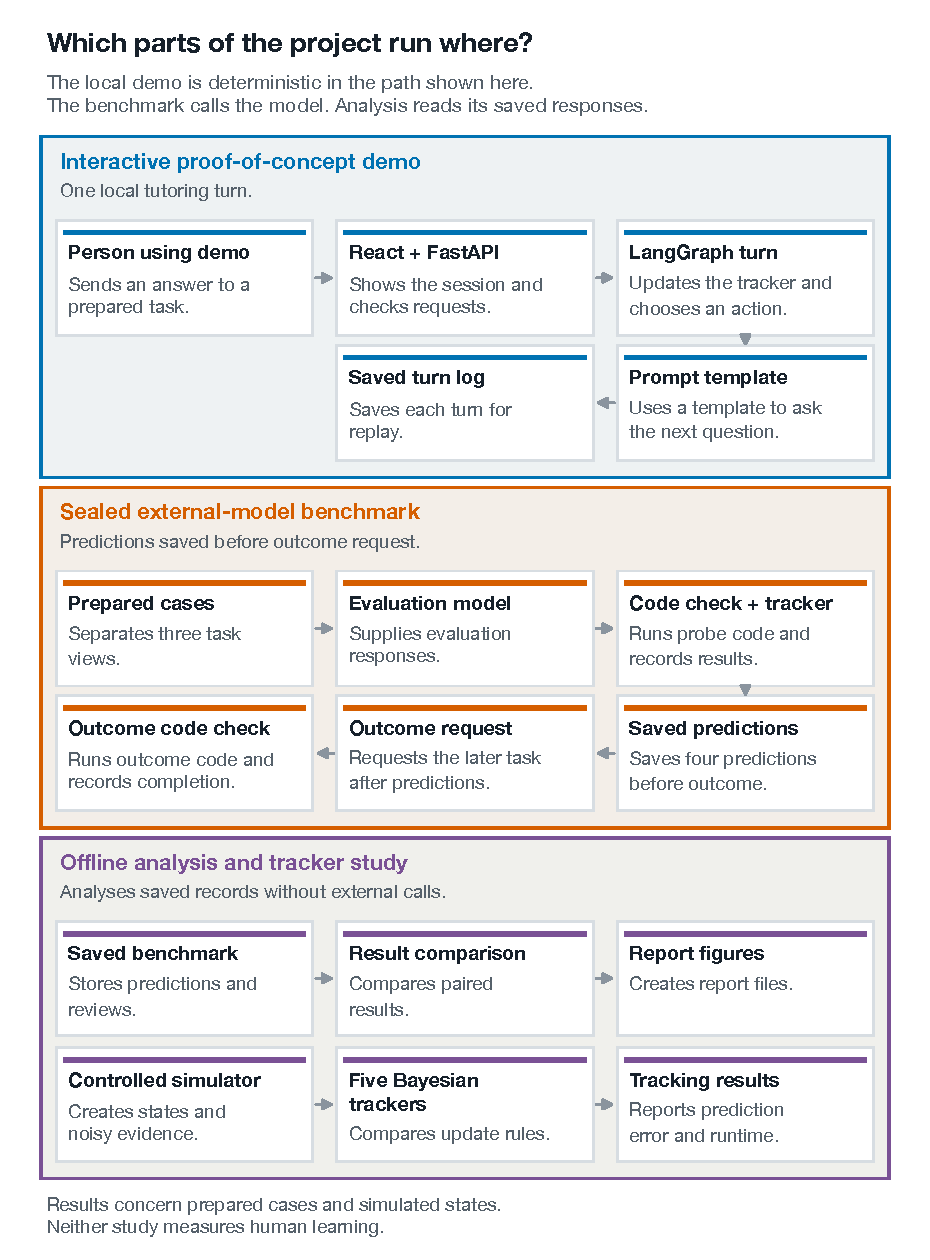
\includegraphics[width=\textwidth]{assets/figures/ch04-system/system_boundaries.pdf}
  \caption{The demonstration, external benchmark and Bayesian tracker study. The top row follows one local tutoring turn.
  The middle row shows the model and sandbox requests, with predictions saved before the outcome request. The bottom row
  shows analysis of saved records and simulated tracker updates. Probe selection and the CSEDM analysis are described separately
  in Chapter~\ref{ch:method}.}
  \label{fig:system-boundaries}
\end{figure}

\section{Engineering Choices}

Pixi fixes the Python and JavaScript environment. FastAPI and Pydantic provide typed API boundaries. React supplies the
examiner-facing interface. LangGraph makes the tutoring state transition explicit. Modal provides an external isolation boundary
for generated code. Saved local artefacts form the scientific record because they can be inspected and replayed without a
hosted dashboard.

\section{The Demonstration Turn}

The local graph makes one pass through evidence classification, tracker update, action selection, prompt generation and a
guardrail check. It has no retry cycle or autonomous planning loop. Each node returns its part of the state, and the final
contract rejects an incomplete result. A task and tracker with different concept identifiers are rejected before execution.

The classifier uses authored text markers. For configured follow-up questions, it uses the current tutor prompt to select
the applicable checks. On the initial question, a reply that matches an output marker but no explanation marker receives an
incomplete category.
The action policy then requests clarification. A recognised misconception receives a hint, while a recognised correct answer
leads to a transfer question. These categories describe matches to the configured rules. Unrecognised phrasing can leave a
valid answer unclassified, so the checker requires manual review of the intended demonstration paths.

The action policy receives the evidence category and observation number. It changes an uncertain observation to a
clarification action when the observation number exceeds three. The tracker score is displayed for inspection but does not
determine the action. Prompt generation uses the action, evidence category, current question and observation count to select
authored text. This provides a repeatable interaction for demonstrating the application. Its classification rules and score
changes have not been validated as measures of learner understanding.

\section{Prediction and Outcome Boundaries}

The benchmark gives the prediction process and evaluator different views of the case records. The prediction process receives
the visible evidence and initial tracker state. Its four conditions begin from the same state after the first answer. The
evaluator receives the later task outcome and uses it to score each prediction.

The system first checks that the input recordings contain no later task responses. It verifies the input hashes, executes
the evidence programs, saves the predictions and records missing cases. It then creates a global decision seal, a record

% TODO: clarify state transition constraints in LangGraph

\chapter{Evidence Tracking and Probe Selection}
\label{ch:method}

An extra coding check can change a prediction, but its result may be unreliable. This chapter explains how the project limits
the influence of one observation and chooses which cases receive a check when the number of checks is restricted. The
simulations make the underlying state and evidence faults known, allowing these decisions to be examined directly.

The final section applies a simpler uncertainty ranking to recorded student activity. It tests whether uncertain predictions
contain a larger share of errors. Together, these methods examine how evidence changes an estimate and where further checking
might be useful.

\section{Bounded Bayesian Updating}

The tracker maintains a probability estimate and revises it after each observation. An ordinary Bayesian update gives more
weight to results that strongly distinguish the two possible states. The modification below limits that weight, because a
faulty check can otherwise cause a large change. The bound controls the size of the update. Whether it improves predictions
is tested in the experiments.

For observation channel $c$, category $z$, and binary state $K_t$, let
$O_c(z,k)=P(Z=z\mid K_t=k,c)$. The state is a binary variable defined by the simulator.
Let $p_t$ be the model's estimated probability of $K_t=1$ before the observation, conditional on the available history.
It need not equal the generating process's conditional probability when the model is wrong. With positive likelihoods,
Bayes' rule gives
\begin{equation}
 p_t^+=\frac{p_tO_c(z,1)}{p_tO_c(z,1)+(1-p_t)O_c(z,0)},
 \qquad
 \frac{p_t^+}{1-p_t^+}=\frac{p_t}{1-p_t}\frac{O_c(z,1)}{O_c(z,0)}.
\end{equation}
Taking logarithms yields the ordinary additive log-odds update. This identity assumes the stated observation likelihoods are
appropriate conditional on the history. Applying several fixed channel likelihoods in succession also assumes the relevant
conditional independence. Correlated evidence can violate that assumption.

The project then modifies the update using fixed trust $0\leq\eta_c\leq1$ and clipping limit $\kappa>0$:

\begin{equation}
  \operatorname{logit}(p_t^+)=\operatorname{logit}(p_t)+
  \eta_c\,\operatorname{clip}\!\left(
    \log\frac{O_c(z,1)}{O_c(z,0)},-\kappa,\kappa
  \right).
\end{equation}

For positive channel likelihoods, an interior prior and non-negative trust, one observation contributes at most $\eta_c\kappa$
to log-odds in absolute value. Across $T$ observations, the sum of the absolute evidence contributions is bounded by
$\sum_{t=1}^{T}\eta_{c_t}\kappa$. Learning and forgetting transitions are separate from this bound.
This is a per-observation bound, not a bound on total movement over a complete episode. Repeated observations can add their
contributions, and the learning and forgetting transitions can also move the estimate. Repeated misleading evidence can
therefore still accumulate substantial influence. Neither calibration nor lower prediction error follows from clipping alone.
The robustness finding is empirical, under the declared simulator.

Equal likelihoods contribute zero. With $\eta_c=1$ and no active clipping, the ordinary Bayesian update is recovered. Otherwise,
the bounded value is a modified belief update and need not be the exact posterior under the original observation model.
The channel-aware variants use category and channel. Their shared input's confidence field is retained but does not multiply
the likelihood again. This is a fixed estimator choice, not learned trust.

The frozen tracker uses $\kappa=2$. Trust weights are 0.50 for public answers, 0.90 for executable probes and 0.40 for
self-explanations. These authored weights limit a single observation's log-odds contribution to 1.0, 1.8 and 0.8 respectively.
They express the study's assumptions about evidence handling and were not estimated from learner data.

The numerical implementation restricts probabilities to $[f_0,1-f_0]$, where $f_0=10^{-6}$, before taking log-odds and
after a non-zero update. The equation above describes the update before this final restriction. For a prior already within
these limits, restricting the result cannot enlarge its movement in log-odds. An input outside those limits is first adjusted.
That adjustment is separate from the bounded evidence contribution. Missing evidence retains the supplied prior.

After the evidence update, the tracker forms the next-turn prior using learning probability $l$ and forgetting probability $f$:
\begin{equation}
 p_{t+1}=p_t^+(1-f)+(1-p_t^+)l.
\end{equation}
This ordering separates evidence about the current state from the subsequent transition. For probabilities in $[0,1]$, the
transition remains in $[0,1]$ as a weighted average. This mechanical property does not validate the transition as a model of
human learning. The implementation applies the numerical probability limits before and after this transition as well.
These transitions apply to the study of bounded updates. The probe selection experiment in
Section~\ref{sec:probe-selection} keeps each case's outcome fixed during selection.

\subsection{Tracker Baselines and Confidence}

The five trackers in the bounded update study differ in how they use an observation. All retain the prior when evidence is missing, before any separate
state transition. The last-observation baseline assigns $1-f_0$ after supporting evidence and $f_0$ after opposing evidence,
where the numerical probability floor is $f_0=10^{-6}$. This deliberately discards the previous estimate.

The hard-BKT baseline uses fixed slip $s=0.15$ and guess $g=0.20$. Its likelihood pair for supporting evidence is
$(1-s,g)$, and for opposing evidence it is $(s,1-g)$, ordered by simulated state $K=1$ and $K=0$.
These parameters are authored rather than fitted to learner records.

For the legacy fractional baseline, let $c\in[0.5,1]$ denote the observation's confidence field, as required by the input contract.
Define $\rho=c$ for supporting
evidence and $\rho=1-c$ for opposing evidence. With fixed $\epsilon=0.15$, the implemented likelihood-like quantities are
\begin{equation}
 \widetilde L_1=(1-\epsilon)^\rho\epsilon^{1-\rho},\qquad
 \widetilde L_0=\epsilon^\rho(1-\epsilon)^{1-\rho}.
\end{equation}
Their contribution to log-odds is therefore
\begin{equation}
 \log\frac{\widetilde L_1}{\widetilde L_0}
 =(2\rho-1)\log\frac{1-\epsilon}{\epsilon}.
\end{equation}
Confidence $c=0.5$ contributes zero. Increasing confidence strengthens the contribution in the category's direction.
This is the frozen transformation, not a calibrated probability of correctness or a claim that confidence specifies a
Jeffrey update. The distinction between evidence strength and a prescribed revised belief is discussed in
\cref{ch:related-work} \parencite{chan2003uncertain}.

The remaining baselines use the channel likelihoods defined above: one applies the ordinary likelihood ratio, while the
bounded variant applies trust and clipping. Neither uses the confidence field. Comparing these trackers thus changes the
observation model as well as, in some comparisons, the update size. Only the channel-aware versus bounded-channel-aware
comparison holds the channel model fixed. Even there, trust weighting and clipping are combined unless separately ablated.

\section{Selecting Probes Within a Fixed Budget}
\label{sec:probe-selection}

Each simulated episode in the probe selection study contains 40 cases. Every ordinary policy sees the same prior estimates and permitted features, then
selects exactly 20 probes before any selected outcome is revealed. The allocation is compulsory, and every selected probe has
the same unit cost. Random selection,
uncertainty-only selection, a plug-in clipped-belief comparator, and the reliability-aware clipped-belief heuristic all spend
the full allocation. Zero or negative scores do not stop selection. Never-probe and always-probe define endpoints. This is
one-step batch selection, without conversational adaptation.

For each case, the simulator draws a starting probability from $\operatorname{Beta}(2,2)$ and clips it to $[0.05,0.95]$.
It then draws $Y_i\sim\operatorname{Bernoulli}(p_i)$ and supplies that same clipped $p_i$ to the policy. Each episode contains
ten families, with one case from each of the four probe classes in every family. Starting
probabilities are calibrated by construction. Held-out environments change evidence reliability, error balance, relevance,
inversion, missingness or dependence. They do not test inaccurate starting probabilities. No learning transition occurs within
a case in this experiment, and the policy cannot inspect the hidden outcome or generating channel rates.

\subsection{Calibration and the Implemented Score}

Sensitivity is the chance that a probe passes when $Y=1$. Specificity is the chance that it fails when $Y=0$. Each has a separate
$\operatorname{Beta}(1,1)$ prior. For $x$ successes in $n$ calibration trials, its posterior is
$\operatorname{Beta}(1+x,1+n-x)$. These trials are simulated from declared channel rates, not collected from students.
Three probe classes use 160 trials per parameter, while the sparse class uses 12. Calibration remains fixed during evaluation.
The dense and sparse high-reliability classes share sensitivity 0.90 and specificity 0.92. The other dense classes use
$(0.78,0.82)$ and $(0.92,0.64)$. Each class contributes ten cases per episode. The shared rates of the first two classes let
the experiment vary calibration sample size while holding their generating reliability constant.

Under symmetric zero-one loss, predicting success incurs expected loss $1-p$, while predicting failure incurs expected loss $p$.
Choosing the smaller gives $R(p)=\min(p,1-p)$ for a coherent probability $p$. This follows the standard posterior expected-loss
decision rule \parencite[Section~5.7, pp.~176--177]{murphy2012machine}.
Let $T_\kappa(p,z;\theta)$ denote the clipped update using sensitivity and specificity $\theta$. The frozen ranking score is
\begin{equation}
 s_i=Q_{0.10,\,\theta\mid D_{\mathrm{cal}}}
 \left[R(p_i)-\mathbb{E}_{Z\mid p_i,\theta}
 R\!\left(T_\kappa(p_i,Z;\theta)\right)\right].
\end{equation}
The implementation uses 8,192 reliability draws with a fixed seed and $\kappa=2$. It takes the lower quantile of these scores
and selects the highest-ranked cases. The plug-in comparator substitutes posterior mean reliability into the same score.
The sample quantile uses linear interpolation. This score averages over pass and fail only. It does not model the probability
of receiving no result. Missing results enter the evaluation environments, where they consume a selected probe and leave its
starting probability unchanged. Thus, the ranking calculation has no explicit penalty for a probe that may return no evidence.
The lower quantile is cautious within the assumed calibration model. It provides no guarantee against failure mechanisms
outside that model.

\subsection{When the Selection Score Overstates the Benefit}

The frozen code and some historical artefacts call these scores EVSI. In this report they are called lower-quantile clipped-risk
scores, because EVSI would suggest a stronger decision-theoretic identity than the implementation has. Clipping generally breaks the correspondence between
the updated belief and the joint model used to average over observations. The score can change when the classification does not.
For $p=0.95$, sensitivity and specificity $0.9$, and $\kappa=2$, passing produces belief $0.992927$ and failing produces
$0.719995$. Table~\ref{tab:acquisition-counterexample} shows the resulting decisions.

\begin{table}[htbp]
  \centering
  \begin{tabular}{@{}lcc@{}}
    \toprule
    Information available & Belief in success & Saved prediction \\
    \midrule
    Before the check & $0.950000$ & Success \\
    Check passes & $0.992927$ & Success \\
    Check fails & $0.719995$ & Success \\
    \bottomrule
  \end{tabular}
  \caption{A counterexample using the frozen clipping bound. The belief changes after either possible check result, but the
  predicted class remains success. The check therefore cannot reduce classification error for this case under the stated model.}
  \label{tab:acquisition-counterexample}
\end{table}

The probability of a pass is $0.86$ and the probability of a failure is $0.14$. The implemented calculation gives

\begin{equation}
  0.05-\left[0.86R(0.992927)+0.14R(0.719995)\right]=0.004717.
\end{equation}

Both branches still predict success, so the actual expected classification error remains $P(Y=0)=0.05$ and its reduction is
zero. A pass moves the belief farther from the threshold, while a failure moves it closer. Weighted by their probabilities,
the risk expression evaluated at those modified beliefs falls below its starting value. The predicted class stays the same
in both branches. This counterexample was found during review after the experiment, using the original clipping bound.
It does not measure how often the issue affected the study's rankings, and is not attributed to the decision-theory reference.

There is a second distinction. Ranking calculates hypothetical updates using each sampled reliability setting. Execution always
updates using the calibration posterior means. The ranking score therefore does not integrate the expected loss of the exact
procedure subsequently executed.

To make the distinction precise, let $\bar\theta$ be the calibration means and
$a_{\bar\theta}(z)=\mathbf{1}\{T_\kappa(p,z;\bar\theta)\geq 0.5\}$. Under generating channel $\theta$, this fixed decision
procedure has expected loss
\begin{equation}
 L_\theta(a_{\bar\theta})=
 \sum_{y\in\{0,1\}}\sum_z P_\theta(Y=y,Z=z\mid p)
 \mathbf{1}\{a_{\bar\theta}(z)\ne y\}.
\end{equation}
Missing observations, where permitted, leave the starting belief unchanged and consume the probe allocation. They must be
included in this sum. The actual expected reduction is $R(p)-L_\theta(a_{\bar\theta})$, assuming the stated joint model.
This is an application of expected-loss evaluation, not a new decision-theory result
\parencite[Section~5.7]{murphy2012machine}. It explains the limitation. It was not substituted into the frozen experiment after
its results were known. The fixed clipped rule can increase expected loss, whereas a Bayes-optimal decision with the option to
ignore an observation cannot do worse in expectation under its own coherent model. That distinction does not provide protection
when the assumed model is wrong.

A decision-aligned calculation would therefore follow four steps for each case:

\begin{enumerate}
  \item Record the classification and expected error before requesting a check.
  \item Enumerate every possible check result, including a missing result where the environment permits one.
  \item Apply the same update and threshold that evaluation will execute. Calculate whether that decision is wrong under
  each possible true outcome.
  \item Average those errors under the stated joint model and subtract the result from the error before the check.
\end{enumerate}

The frozen policy does not implement these four steps as one coherent calculation. They specify the correction required before
a future selector can be described as choosing probes by expected classification-error reduction.

The batch objective introduces a further limitation. With equal probe costs and exactly $k$ selections, taking the largest
$s_i$ maximises the sum of the selected scores. It does not generally maximise a lower quantile of their combined benefit.
For uncertain quantities $X_i$, quantiles do not generally add:
\begin{equation}
 Q_{0.10}\!\left(\sum_{i\in S}X_i\right)
 \ne \sum_{i\in S}Q_{0.10}(X_i)
 \quad\text{in general}.
\end{equation}
Here $S$ is a selected set. Shared uncertainty about channel reliability affects its joint outcome. Even independent quantities
need not satisfy equality. For example, let two independent quantities each equal zero with probability $0.06$ and one otherwise.
Each has lower tenth quantile one, but their sum has lower tenth quantile one, rather than two: the probability of a sum at most
one is $1-0.94^2=0.1164$. This mathematical example is separate from the simulator results.

Consequently, cautious individual rankings provide no established lower-quantile guarantee for the batch's total benefit.
Correcting the individual expected-loss calculation would still leave that distinction to address. The frozen study evaluates
the ranking rule as implemented. Optimal selection under joint reliability uncertainty remains unestablished.

The reference labelled \texttt{oracle} uses true channel rates but retains the assumed update and clipped-belief risk score.
It is a true-channel reference, not an optimal accuracy bound. Historical policy identifiers remain unchanged for reproduction.
The final evaluation measures classification errors against generated outcomes separately from the acquisition score. Those
measurements describe the implemented heuristic, not a correctly integrated value-of-information optimiser.

\subsection{How the Equations Are Implemented}

Table~\ref{tab:acquisition-implementation} maps each calculation to its code. Paths start at
\path{development/src/socratic_tutor/acquisition_study/}.
\begin{table}[htbp]
 \centering
 \begin{tabularx}{\textwidth}{@{}>{\raggedright\arraybackslash}p{0.25\textwidth}>{\raggedright\arraybackslash}X@{}}
 \toprule
 Quantity & Implementation and interpretation \\
 \midrule
 Ranking score & \path{policies.py}: \texttt{reliability\_aware\_evsi\_scores} is the historical function name. It computes a lower quantile of changes in clipped-belief risk. \\
 Executed update & \path{evaluation.py}: selected observations update using calibration means, without reranking. \\
 Measured error & \path{evaluation.py}: final thresholded prediction compared with \texttt{latent\_success}. \\
 Primary interval & \path{primary_analysis.py}: paired episode resampling with a fixed calibration fit. \\
 \bottomrule
 \end{tabularx}
 \caption{Where the probe selection calculations are implemented. The ranking score uses a risk expression evaluated at modified
 beliefs. Measured error counts incorrect final predictions. A higher ranking score need not produce fewer errors.}
 \label{tab:acquisition-implementation}
\end{table}

\subsection{Failure Settings and Their Limits}

\Cref{tab:acquisition-faults} describes the seven stress tests in \path{v1-environments.yaml}.
For sensitivity or specificity $r$, scaling by $s$ gives $0.5+s(r-0.5)$ before inversion.

\begin{table}[htbp]
 \centering
 \begin{tabularx}{\textwidth}{@{}>{\raggedright\arraybackslash}p{0.23\textwidth}>{\raggedright\arraybackslash}X@{}}
 \toprule
 Setting & Constructed change and purpose \\
 \midrule
 Matched & Uses the calibration-generating channel rates to check behaviour when the assumed channel family is appropriate. Finite calibration samples still introduce estimation error. \\
 Lower reliability & Scales both rates' distance from chance by 0.5 to test overconfidence in channel quality. \\
 Asymmetric errors & Scales sensitivity's distance from chance by 0.2 and leaves specificity unchanged to test excess false negatives. \\
 Irrelevant evidence & Sets sensitivity and specificity to 0.5 to test evidence carrying no information about the target. \\
 Inverted evidence & Reverses every sampled result to test a fully reversed observation channel. \\
 Missing results & Missing probability is $0.05+0.55(1-2|p-0.5|)$, capped at 0.60. Lost observations concentrate near uncertain priors. \\
 Family failures & Reverses all four outcomes in a family together with probability 0.30 to test shared corruption. \\
 \bottomrule
 \end{tabularx}
 \caption{Authored acquisition stress settings. The probabilities were chosen to specify controlled experiments. Their values
 do not estimate the frequency of software faults or learner behaviour.}
 \label{tab:acquisition-faults}
\end{table}

The v1 evaluation motivates checking evidence quality, but its observed defects do not establish these probabilities or validate
each mechanism. In particular, full inversion is a deliberately severe control. The missingness variable is proximity to prior
probability one half, not an observed measure of student difficulty.

The broader concern about acquisition under wrong model assumptions is supported by existing work. For example,
\textcite{tang2026robust} analyse error amplification under model misspecification and propose an acquisition criterion that
accounts for it. That work provides related theoretical context. This study does not implement its criterion or transfer its
guarantees to clipped-belief selection.

The matched setting is a project-authored implementation check. Lower reliability and
asymmetric errors are project-authored parameter shifts. Irrelevance and full inversion are project-authored contrastive controls.
Missingness and family corruption are project-authored structural stress conditions. Their immediate specification source is the
frozen configuration, and their purpose is stated in \cref{tab:acquisition-faults}. Neither the cited literature nor v1 supplies
their numerical rates. This distinction avoids presenting plausible failure stories as observed educational data.

Family corruption changes marginal reliability as well as dependence: a base rate $r$ becomes $0.3+0.4r$ after random family
inversion. Without an independent-corruption condition at the same marginal rates, that setting cannot isolate the causal effect
of correlation alone. Its result concerns the combined failure mechanism. No additional control was added after viewing results.

\subsection{Comparison and Uncertainty}

Development checks used 50 episodes per environment. The final comparison used 2,000. The frozen plan permitted one final
evaluation and exact retries, while prohibiting parameter selection from evaluation outcomes or use of those outcomes to
update reliability. Its software-failure rule required invalidating the affected run, fixing the version and rerunning.
Development ablations and calibration sensitivity remain diagnostic analyses, with their own records and denominators.

The acquisition extension had a planned 40-hour technical limit to protect time for writing and verification. This records
the intended scope. The retained experiment reports do not independently establish the total working hours spent. The later
mathematical review corrected interpretation of the saved results without replacing the evaluated method.

A proposed replay of the acquisition policies over the external-model benchmark was dropped. Those records did not contain
the corresponding reliability inputs available before the outcomes were known. Constructing them retrospectively would make
the comparison depend on choices informed by those outcomes. The external benchmark therefore motivates the acquisition
study. It does not provide an external validation of the selector. Replaying saved benchmark responses to check the original
scoring remains a separate operation.

Before the final simulator run, a reviewer with self-described machine-learning experience assessed the design packet and
environment descriptions. The disposition records 6 September 2026. The reviewer reported working independently, without
seeing development outcomes or policy rankings, and recommended proceeding unchanged. They nevertheless marked uncertainty
about omitted failure types, inference of the hidden environment and the episode as an independent unit. These reservations
remain limitations. The recommendation does not resolve them or validate the simulator as a model of learners.

The packet and response were not committed separately, so Git history alone cannot establish their order. The retained
response and disposition document the reported process. Information isolation applies to the fixed, inspected policies.
Arbitrary code can still read local files. Episodes are the resampling unit because failures
may be shared within their case families, while separate episodes use independent random draws. This is an assumption of
the simulation design, rather than an empirical finding from the review.

The primary comparison equally weights six specified mismatch environments, with 2,000 episodes per environment.
Pairing is preserved within each environment. The three primary comparisons use Bonferroni-adjusted percentile-bootstrap
intervals from 20,000 draws. These intervals are conditional on the frozen calibration fit. They do not include variability
from collecting another calibration sample. The separate 20-seed development sensitivity analysis does not change that scope.

The success rule requires favourable aggregate intervals against all three comparators and no adverse per-environment point
estimate against the plug-in comparator. This is the prespecified study criterion. A point estimate cannot rule out meaningful
harm, so the rule is not a per-environment safety guarantee. Equal weighting describes the chosen stress-test mixture, not
deployment prevalence. The candidate failed this rule. The threshold and comparators remained fixed.

\section{Prediction from Historical Learner Records}

The exploratory analysis uses the CSEDM 2019 Data Challenge, version 1.1, which documents novice Python programming records and ten student-separated
evaluation folds \parencite{csedm2019challenge}. The local inventory identifies the analysed archive by its SHA-256 checksum.
The separate Java CodeWorkout release is excluded. Each target's learner-history features use only that learner's earlier events. Preprocessing is fitted within
the training fold. Overall prevalence, problem frequency, and a fixed learner-history logistic model produce out-of-fold
predictions. The primary model uses earlier activity, submission, correctness, hint-request and distinct-problem counts or rates,
plus training-learner success on the target problem. The latter excludes the target's own label for training rows. Test features
use training-fold statistics only. Missing values use training medians and indicators. Numeric scaling is fitted on training data.
Problem success rates use the available training-fold labels without a global calendar cut-off. The evaluation therefore
tests prediction for learners excluded from model fitting on the existing problem set. It does not recreate deployment in
which only records collected before a particular date are available for training.

The chronology boundary is strict: an event contributes features only when its \texttt{Order} is less than the target's
\texttt{StartOrder}. The supplied \texttt{FirstCorrect} value is the outcome, never an input. The source defines the target
as first-attempt success without requesting a hint \parencite[The Data, Predict.csv]{csedm2019challenge}. This study uses
that supplied label rather than reconstructing it from later events. The target's later correctness,
hint use and attempt count are also excluded. Learners could attempt problems in different orders, so problem identity alone
does not establish which events were available at prediction time.

The source documentation notes that activity correctness was reconstructed after the original study and may differ from the
feedback learners received. Version 1.1 also corrected leakage in the supplied example model. This dissertation uses its own
fold-specific pipeline. Reproducing the supplied example's metrics checks agreement with that reference. The documented data
limitations still apply. The local inventory retains unavailable activity correctness values. They are excluded from
correctness-rate denominators while activity counts retain the events.

The predictor uses scikit-learn \parencite{pedregosa2011scikit}. The locked environment specifies the installed version.
The frozen \path{v1-analysis.yaml} CSEDM plan specifies logistic regression with an intercept, L2 regularisation and inverse
regularisation strength $C=1$. Training uses the \texttt{lbfgs} solver, no class weighting, at most 1,000 iterations, and tolerance
$10^{-8}$. The recorded random seed is 9052901. The implementation treats a convergence warning as a failed run rather than
silently accepting an unfinished fit. These settings are fixed. There is no hyperparameter search, fitted probability calibration,
or model selection based on test-fold results.

Probabilities at or above 0.5 predict first-attempt success. The separate uncertainty ranking uses $|p-0.5|$ in ascending order.
Small values mean the classifier is near its decision threshold. This is a simple ranking score, not a full estimate of model
uncertainty or a guarantee that a probability is calibrated. Equal scores are ordered by a stable hash of the fold, learner,
problem and prediction cut-off identifiers, without using the outcome.

For fold $f$ with $N_f$ targets, selection takes $k_f=\lfloor0.5N_f\rfloor$ predictions closest to probability $0.5$.
This selects 361 of 729 targets, rather than the 364 from a single global allocation. If $E_f$ is the fold's error count, expected
random error capture is $\sum_f k_f E_f/N_f$. Dividing this by $\sum_f E_f$ gives the random captured-error recall used in the
primary comparison. The observed recall uses the actual number of selected errors instead.

Accuracy, Brier score, log loss and calibration error are secondary descriptions. Log loss clips probabilities at $10^{-6}$
and $1-10^{-6}$. Calibration error uses ten equal-width bins. Leave-one-fold-out summaries check whether omitting a single fold
changes the primary pattern. They do not retrain models or create independent replications.

The 10,000-draw bootstrap resamples learners, retaining all their rows and the original predictions and selections. Its interval
is conditional on those fitted predictions and selections. Models are not refitted and cases are not reranked. The original
fold selection probabilities $k_f/N_f$ are also held fixed when calculating the resampled random comparator. Shared training
sets across folds create further dependence that learner resampling does not fully represent. The analysis concerns the existing
learners and problems. It establishes neither unseen-problem generalisation nor whether reviewing an error would correct it.

\chapter{Evaluation}
\label{ch:evaluation}

\section{External-Model Study and Harness Correction}

After correction, executable evidence improved one of 23 eligible predictions and caused no regressions, an observed gain of
4.35 percentage points. Related and unrelated passing evidence produced identical binary decisions. The corrected result
leaves a useful benefit unresolved and provides no evidence that this tracker recognised the relevance of a passing check.

The original sealed analysis suggested a 30.43 percentage-point advantage over dialogue alone. Its paired interval was wide
and the exact McNemar comparison was not significant. A full replay then found that the test harness had compared equivalent
sequence values incorrectly. Nineteen of 48 execution records changed:
12 evidence labels and five criterion labels changed, one further criterion record changed its test counts while remaining
unsuccessful, and one missing criterion was reclassified from sandbox error to invalid submission. Thus, 17 binary labels
changed. The count of 19 also includes a test-count change and a failure-status correction.

The corrected 95\% paired case-bootstrap interval was 0.00 to 13.04 percentage points, and the two-sided exact McNemar
test gave $p=1.0$. Only one case had different correctness outcomes between the conditions: evidence corrected that prediction,
while 18 cases were correct under both conditions and four were incorrect under both. The original exact comparison gave
$p=0.0923$. Neither result establishes equivalence. In particular, the corrected interval still includes the declared
ten-percentage-point threshold for a practically meaningful improvement, although the point estimate falls below it.
The experiment therefore leaves a meaningful benefit unresolved. It cannot show that probing has no useful effect.
These intervals describe resampling this small authored corpus and do not account for its shared concept families or a fresh
model run. Figure~\ref{fig:harness-correction} shows how the correction changed the estimated advantage and its interval.

Here, performance means passing the authored criterion checks. Repairing the sequence comparison did not establish that those
checks covered every task requirement. The worked example retains a known coverage limitation: checking returned values did not
establish that the supplied list was changed. The corrected analysis remains a comparison against this limited instrument.

\begin{figure}[tb]
  \centering
  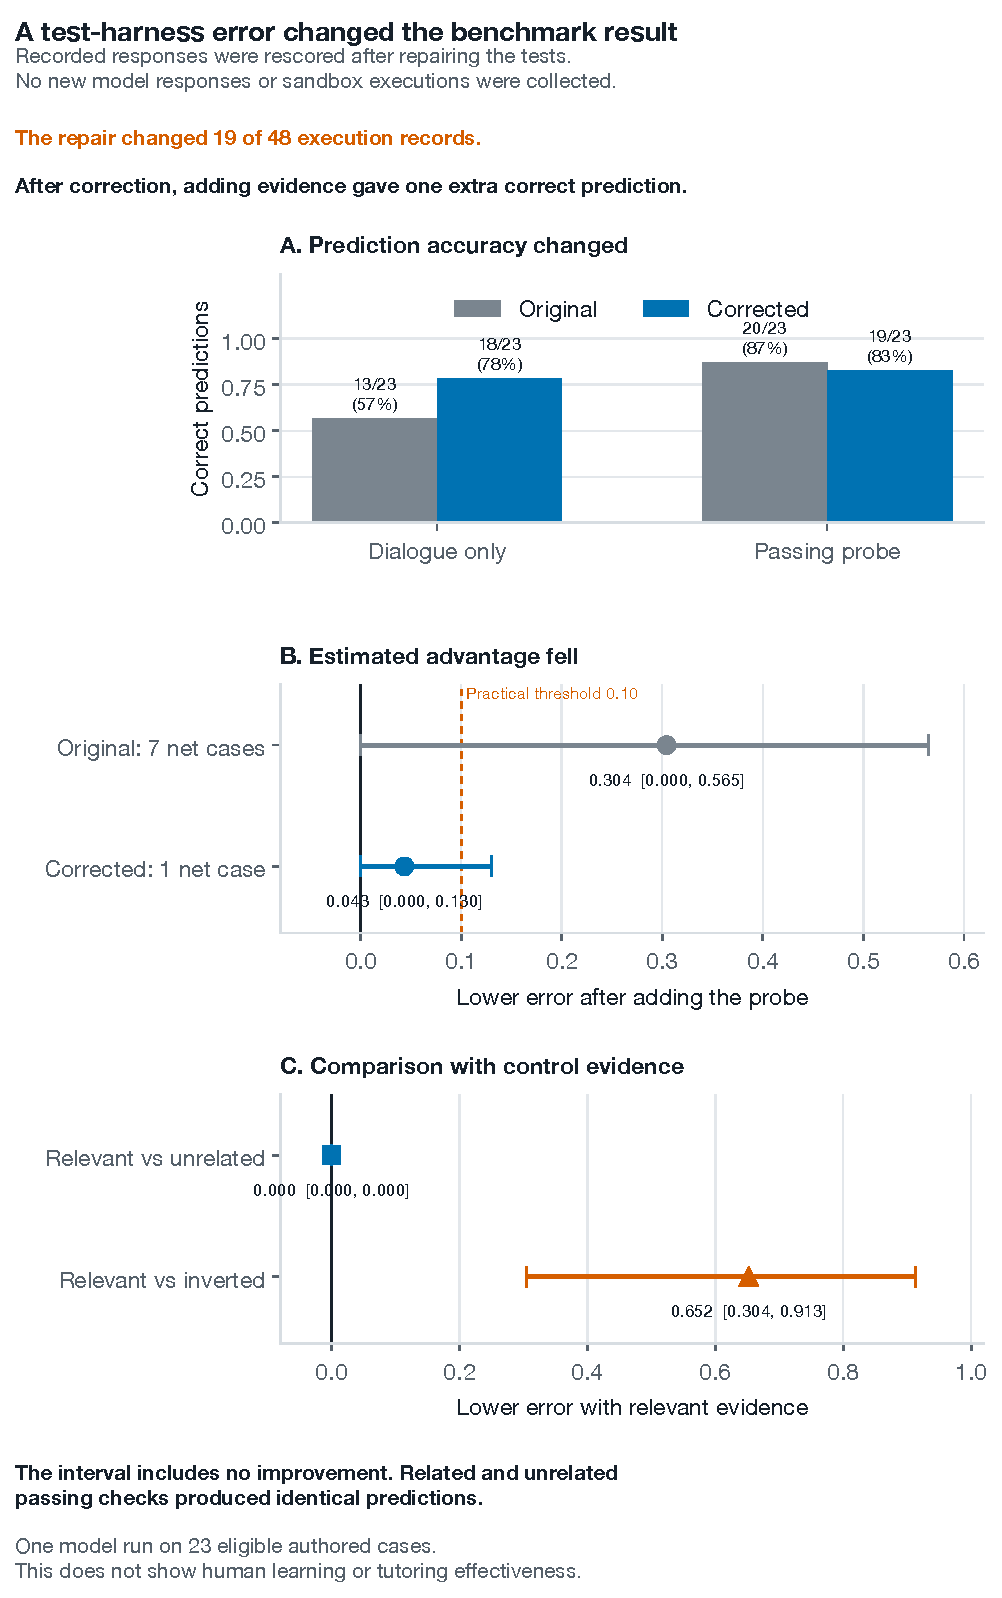
\includegraphics[width=\textwidth,height=0.82\textheight,keepaspectratio]{assets/figures/ch06-evaluation/harness_correction_result.pdf}
  \caption{Effect of correcting the test harness on 23 eligible authored cases. Adding executable evidence to the dialogue
  increased correct predictions from 13/23 to 20/23 under the original scoring, and from 18/23 to 19/23 after correction.
  The corrected reduction in classification error was 4.3 percentage points (95\% paired bootstrap interval: 0 to 13.0).
  Positive differences favour adding evidence. Related and unrelated passing checks produced identical predictions.
  The correction reuses one recorded run. It does not measure learning.}
  \label{fig:harness-correction}
\end{figure}

\subsection{The Missing Criterion Outcome}

Case \texttt{h-c2m2-03} has no valid binary criterion outcome. The original execution was recorded as a sandbox error.
The corrected replay records an invalid submission. Neither status is an observed test failure, so the case remains excluded
from the 23-case primary analysis.

Its saved dialogue-only and valid-evidence predictions both indicate success. If a valid criterion outcome had been failure,
both would be wrong. If it had been success, both would be right. Holding the saved predictions and all other outcomes fixed,
the two hypothetical completions give 18/24 versus 19/24 correct predictions, or 19/24 versus 20/24. In either case, the
valid-evidence advantage would be $1/24$, or 4.17 percentage points. The missing case cannot add a disagreement between these
two conditions under either binary completion. Their observed advantage remains $1/23$, or 4.35 points.

This is a descriptive sensitivity calculation, not an imputed observation or a new primary analysis. It does not justify
treating invalid submissions as failures, assuming that missingness is random, or extending the finding beyond the authored
cases. The corrupted-evidence prediction for this case is failure, so the same cancellation does not apply to every secondary
comparison. The small corpus, shared concepts and single model run remain separate limitations.

For the secondary comparisons, valid and unrelated evidence have identical predictions on all 24 cases, including the missing
case. Their difference therefore remains zero under either binary completion. Valid evidence exceeds corrupted evidence by a
net 15 correct predictions among the 23 observed cases. Adding a hypothetical failure for the missing case reduces that net
difference to 14. Adding a success increases it to 16. Across 24 cases, these alternatives give advantages of 58.33 and
66.67 percentage points, respectively (the observed 23-case difference is 65.22 points).

The frozen combined control contrast averages the valid-versus-unrelated and valid-versus-corrupted differences. Its observed
value is 32.61 percentage points. The two hypothetical completions give 29.17 and 33.33 points. These describe alternative
completions of the missing outcome. The positive combined contrast comes entirely from the corrupted-evidence comparison.
It cannot establish that relevant evidence helps more than unrelated evidence. No secondary outcome is filled in, and the
frozen analyses retain their original 23-case denominator.

\subsection{Reviewer Agreement and Its Limits}

The two public-answer reviewers agreed on all 24 cases. Both assigned 23 answers to the correct category and one to the
conflicting category. No disagreement required adjudication. Raw agreement and unweighted Cohen's kappa were both 1.0.
These ratings concern the visible answers, not the later criterion outcomes. With four of the six categories unused, this
sample provides little evidence about how consistently the reviewers would distinguish the full category set.

The separate failure review covered six records, assessed by the author and an independent reviewer. Both final submissions assigned four to item ambiguity or test defect and
two to no observed failure. Raw agreement and kappa were again 1.0, with no adjudication required. These six records are a
selected diagnostic set, not a random sample of all possible failures. Their category counts cannot estimate a general failure
rate or establish that every relevant defect was found.

The archived author sheet contains an earlier version with three different categories. The agreement calculation uses the
revised author sheet and the final independent submission. It therefore describes agreement after revision. It does not
establish agreement between initial judgements or show whether the revision process affected their convergence.

Agreement shows that the submitted categories matched. It does not prove that they were correct, that test coverage was complete,
or that the chosen category identifies a unique cause. A shared taxonomy can encourage a shared interpretation. The reliability
reports summarise final submissions. Preserved review records are needed to inspect their revision
history. The complete harness correction remains separate execution evidence and must not be inferred from agreement alone.

\subsection{Recorded Workload and Missing Measurements}

The original external run recorded 72 Cerebras responses: 48 across the public-answer and evidence channels, followed by
24 criterion responses. Their total usage was 15,899 input tokens and 16,684 output tokens. Summed provider latency was
32.70 seconds. This is the sum of individual recorded request latencies, not elapsed experiment time or the waiting time of a
student using the tutor. Response-capture spans were about 633 seconds for decision generation and 364 seconds for criterion
generation, in separate phases.

Of 48 original sandbox execution attempts, 47 completed: all 24 evidence executions and 23 of 24 criterion executions.
The missing criterion left 23 cases eligible for paired analysis. Completion is distinct from passing a test. Subsequent
harness correction reused recorded model responses. It did not constitute another independent model evaluation.

Provider charges were not reported. Sandbox duration, CPU use and memory use were also absent from the original records.
These quantities remain unavailable, rather than being treated as zero. The original reconciliation report also predates the
complete harness correction. Its partial corrected pass/fail tallies are superseded. Only its original workload accounting is
used here.

An evidence-informed condition required the public response plus an additional model response and sandbox execution. Criterion
generation was an evaluation requirement, not an input available to a deployed prediction rule. This accounting establishes
extra experimental work, but not realised financial savings, a minimum-cost selection policy, or faster classroom tutoring.
The probe selection simulator performs no provider or sandbox call, and its probe allocation cannot fill these missing cost measurements.

\FloatBarrier
\section{Bounded Update Study}

Across five adverse simulator conditions, the bounded tracker had mean Brier error 0.0094 lower than ordinary channel-aware Bayes.
The paired 95\% interval was $[-0.0101,-0.0086]$. Under clean evidence, bounding increased Brier error by 0.0033, and the upper
interval bound of 0.0042 remained below the fixed 0.0100 tolerance. Figure~\ref{fig:tracker-result} shows the comparison
across the tested conditions.

The favourable adverse-condition average hides differences between conditions. Bounded updating reduced Brier error under
uninformative, inverted and reliability-misspecified evidence, but increased it under missing and contradictory evidence.
It passed the declared rule for average improvement and the permitted loss under clean evidence. This is
an empirical result, separate from the per-observation bound on log-odds movement.

\begin{figure}[tb]
  \centering
  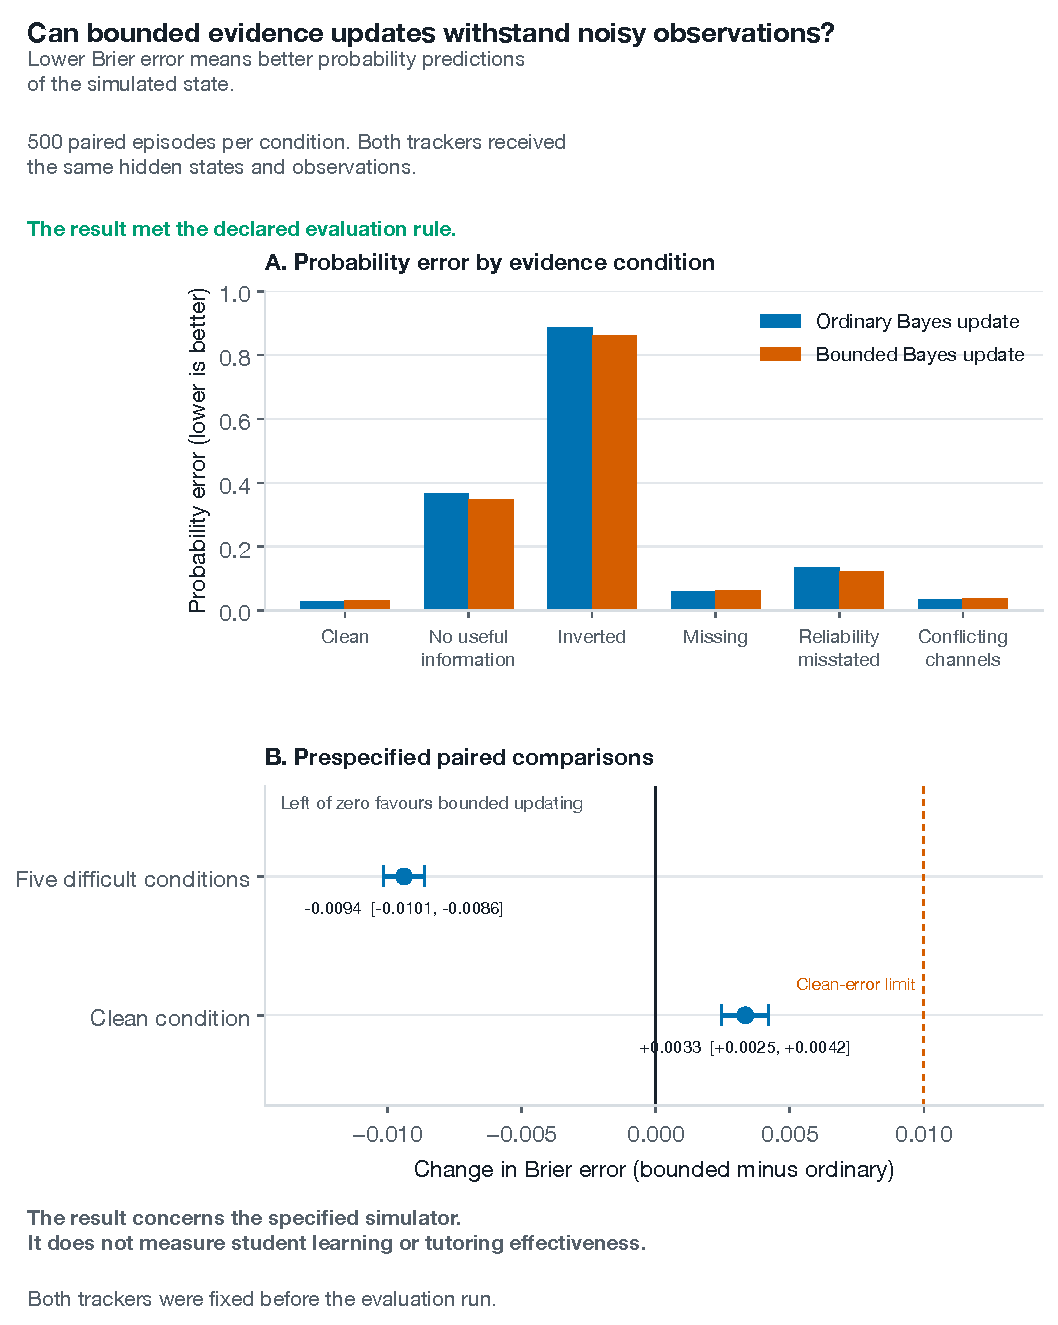
\includegraphics[width=\textwidth,height=0.82\textheight,keepaspectratio]{assets/figures/ch06-evaluation/tracker_study_canonical.pdf}
  \caption{Ordinary and bounded Bayesian updates across 500 matched simulated episodes per condition. Lower Brier error
  indicates better probability predictions. Differences are bounded minus ordinary. Negative values favour bounded updating.
  Paired 95\% intervals describe the equally weighted average across five adverse conditions and the clean condition.
  Bounded updating improved the adverse average, while error increased under missing, contradictory and clean evidence.
  The results concern the specified simulator. They do not measure student learning.}
  \label{fig:tracker-result}
\end{figure}

\FloatBarrier
\section{Selective Acquisition Study}
\suppressfloats[t]

At the fixed 50\% budget, the proposed policy reduced held-out classification error by 1.19 percentage points relative to random
selection. It increased error by 0.855 percentage points (0.86 when rounded to two decimal places) relative to uncertainty-only
selection and by 0.54 points relative to the plug-in
clipped-belief comparator. All three multiplicity-adjusted intervals excluded zero. The proposed policy therefore failed the declared
all-comparator rule.

The budget was compulsory: every selector that could probe selected 20 of the 40 cases. The candidate therefore chose the
allocation, rather than deciding whether an additional check was worth requesting in the first place. The comparison
concerns which cases were checked under this fixed design. Every selector requested the same number of checks.

These are measured errors of the implemented heuristics. As Chapter~\ref{ch:method} explains, the acquisition score is not
generally expected classification-error reduction. The result therefore cannot establish the performance of an exact
value-of-information optimiser. The counterexample identifies a limitation. It does not quantify its contribution to the
observed ranking differences.

The intervals are conditional on the frozen calibration fit and refer to the equally weighted six-environment comparison.
They do not include calibration-sample variability or establish safety in every environment. Starting probabilities were
calibrated by construction, and each policy selected its entire allocation before seeing probe outcomes.

The plan divides the 5\% error allowance among three primary comparisons, giving each a nominal
$1-0.05/3=98.33\%$ interval. This targets at least 95\% joint coverage if each interval achieves its stated coverage. It does
not mean that the set has 98.33\% joint coverage. The adjustment does not require independent comparisons, but it cannot
repair inaccurate marginal bootstrap coverage or include variation omitted by the resampling procedure.

\Cref{tab:m7b-primary-comparison} reports the frozen primary comparison using the corrected method names. The plug-in
comparator uses mean reliability in the same clipped-belief scoring rule. Ordinary expected-loss selection remains untested.

% Values checked against canonical_primary_analysis_report.json, hash
% edec72e5a8764d4df5e52c5c09a1de213efeb3e22d4c5972708ec441e70a9d34.
\begin{table}[htbp]
  \centering
  \begin{tabularx}{\textwidth}{@{}>{\raggedright\arraybackslash}Xrr@{}}
    \toprule
    Comparator & Error (\%) & \shortstack{Difference [interval]\\(percentage points)} \\
    \midrule
    Random selection & 34.45 & $-1.19\;[-1.33,-1.05]$ \\
    Highest uncertainty & 32.41 & $+0.86\;[+0.76,+0.95]$ \\
    Plug-in clipped-belief rule & 32.72 & $+0.54\;[+0.48,+0.60]$ \\
    \bottomrule
  \end{tabularx}
  \caption{Primary prediction errors at the fixed 50\% probe allocation, averaged equally across six held-out simulated
  settings (2,000 paired episodes per setting). The candidate's error was 33.26\%. Differences are candidate minus comparator.
  Negative values favour the candidate. The planned 98.33\% intervals adjust for three comparisons and hold calibration fixed.}
  \label{tab:m7b-primary-comparison}
\end{table}

For the proposed policy, matched-setting error fell from 31.23\% with no probes to 14.54\% when every case was probed. Across the
six held-out settings, the equally weighted error rose from 31.23\% to 37.66\%. Irrelevant and inverted evidence produced the
largest harm. This descriptive budget analysis shows why success under the policy's own assumptions was insufficient.
At the full allocation, selection no longer distinguishes the ordinary policies: every case is probed and the same bounded
update is applied. Harm at this endpoint concerns evidence updating under the declared faults, rather than the ranking alone.
The equal-weight average is not an estimate of how often those faults occur in deployed systems.

\begin{table}[htbp]
  \centering
  \begin{tabular}{@{}lrrr@{}}
    \toprule
    Setting & No probes (\%) & Full probing (\%) & Change (points) \\
    \midrule
    Matched & 31.23 & 14.54 & $-16.69$ \\
    Lower reliability & 31.15 & 29.08 & $-2.07$ \\
    Asymmetric errors & 31.16 & 27.33 & $-3.83$ \\
    Irrelevant evidence & 31.52 & 43.14 & $+11.62$ \\
    Inverted evidence & 31.17 & 71.89 & $+40.73$ \\
    Missing results & 31.18 & 22.71 & $-8.47$ \\
    Family failures & 31.18 & 31.84 & $+0.66$ \\
    \bottomrule
  \end{tabular}
  \caption{Descriptive endpoint errors from the frozen secondary budget analysis, with 2,000 episodes per setting.
  Lower error is better. Changes are calculated before rounding, so displayed endpoint subtraction may differ by 0.01 points.
  The endpoints use identical updating across ordinary selectors. This table does not compare their ranking quality.}
  \label{tab:acquisition-endpoints}
\end{table}

\Cref{tab:acquisition-endpoints} shows why the held-out average needs its individual settings. Lower reliability, asymmetric
errors and missing results retained improvements at full probing. Irrelevance, inversion and family corruption worsened error.
The inverted setting had the highest full-budget error, 71.89\%, under deliberately complete reversal of the observation channel.
These endpoint differences are descriptive, without new significance claims or thresholds. Family corruption changes marginal
reliability as well as dependence, so its difference cannot be attributed to correlation alone.

\subsection{Where the Fixed-Budget Selector Lost}

At the primary 50\% allocation, the candidate's mean error exceeded both informed comparators in all seven environments,
including the matched check. In that matched setting, its error was 19.18\%, compared with 18.12\% for uncertainty-only
selection and 18.38\% for the plug-in clipped-belief rule. Thus, a channel model matching the calibration-generating process
was not sufficient for the candidate to lead these comparisons.

Among held-out settings, asymmetric errors produced the largest candidate disadvantage against uncertainty-only selection
($+1.10$ percentage points) and the plug-in rule ($+0.80$ points). Inverted evidence produced the highest candidate error at
50\%, 53.80\%, and the only setting in which its point estimate was worse than random selection ($+2.19$ points).
The candidate therefore beat random on the held-out average while still losing to it under full inversion.

These values come from the frozen primary per-environment effect table. They describe the location of the losses. The
simultaneous inferential comparisons concern the held-out aggregate reported above. The fact that each point estimate favours
an informed comparator is not a separate claim of statistical significance for every environment. Nor does this breakdown
identify which component of the candidate caused its disadvantage.

\subsection{Development-Only Component Comparison}

The frozen development ablation compared four combinations of reliability scoring and updating. Each used 20 probes per episode,
with 50 episodes in each of the six held-out settings. These results are diagnostic and were not used to select the canonical
method. Table~\ref{tab:acquisition-ablation} reports the four combinations. They must not be pooled with the 2,000-episode
canonical comparisons.

\begin{table}[htbp]
  \centering
  \begin{tabular}{@{}lrr@{}}
    \toprule
    Reliability used for ranking & Bounded update & Unbounded update \\
    \midrule
    Lower-quantile score & 33.30\% & 33.40\% \\
    Plug-in mean reliability & 32.95\% & 33.07\% \\
    \bottomrule
  \end{tabular}
  \caption{Mean classification error from 50 development episodes in each of six simulated failure settings, with 20 probes
  per 40-case episode. Settings receive equal weight. Lower values are better. These are descriptive development results.
  Clipping is applied or removed in both hypothetical scoring updates and executed updates. Consequently this comparison does
  not isolate its effect on ranking from its effect on the final belief.}
  \label{tab:acquisition-ablation}
\end{table}

With lower-quantile scoring, clipping reduced mean error by 0.10 percentage points. With mean-reliability scoring, it reduced
error by approximately 0.12 points. The difference between these effects was $+0.017$ points, calculated before rounding.
This small descriptive interaction provides no clear evidence that the two components worked especially well together.
Replacing lower-quantile scoring with the plug-in rule reduced error by 0.35 points when bounded and 0.33 points when unbounded.
No inferential interaction claim follows from this development report.

The comparison preserves the implementation's score definitions. In particular, the plug-in row evaluates the score at mean
reliability. It does not average scores over the reliability posterior. These ablations help locate differences between the
implemented variants, without establishing a general result about conservative acquisition or Bayesian decision theory.

\subsection{Development Sensitivity and Reliability Control}

The separate calibration sensitivity used 20 prespecified calibration seeds while retaining the development evaluation design.
The candidate's held-out error estimate was lower than random selection for all 20 seeds, lower than uncertainty-only selection
for none, and lower than the plug-in comparator for one. No seed satisfied the complete robustness pattern. Candidate-minus-
comparator differences ranged from $-2.24$ to $-0.74$ percentage points against random, $+0.09$ to $+0.89$ against uncertainty,
and $-0.03$ to $+0.55$ against the plug-in rule. These ranges describe the specified seeds, not confidence intervals or a
distribution over all possible calibration datasets. They did not select the canonical calibration fit.

The reliability control used one frozen reassignment of reliability summaries between probe classes during ranking. Both
selectors faced the same development episodes. Executed updates retained each selected case's original calibrated reliability.
Across 50 episodes per held-out setting, candidate mean error was 33.30\%, compared with 33.37\% under the reassignment.
The difference was approximately $-0.067$ percentage points. The candidate was worse under inversion by 1.20 points, despite
the small average advantage.

This control checks the effect of that particular mismatch between ranking inputs and case identity. It is not a test over all
permutations, a probability that reliability information is useful, or proof of equivalence between the selectors. Both the
control and calibration sensitivity are development-only diagnostics. Their patterns are consistent with the canonical failure
to beat both informed comparators, but they do not enlarge the canonical sample or its interval coverage.

\FloatBarrier
\section{Historical CSEDM Companion}
\suppressfloats[t]

The learner-history logistic model produced 195 errors over 729 out-of-fold predictions, with accuracy 0.733. The problem-frequency
baseline produced 200 errors and accuracy 0.726. Selecting the most uncertain 361 predictions captured 141 of the 195 logistic
model errors, compared with an exact random expectation of 49.54\%. The gain was 22.77 percentage points. Its learner-bootstrap
95\% interval was 16.41 to 28.98 points. Figure~\ref{fig:csedm-result} shows the share of errors captured by each selection
approach and the difference between them.

Selection took half of each test fold, rounded down. This was an offline ranking calculation. No reviewer intervention was
performed. The interval resamples learners while retaining the fitted predictions and original selections, so it is conditional
on the fitted models and selected rows. It does not include refitting or reranking variability. The study supports error
prioritisation on the existing problem set, without showing that subsequent review would correct those errors or that the
finding extends to unseen problems.

% Generated from the frozen aggregate CSEDM analysis report.
\begin{table}[tb]
\centering
\caption{Prediction results on 729 historical targets from 86 learners and 19 Python problems.
Each learner was evaluated using models fitted on other learners. Higher accuracy and lower errors,
Brier score, log loss and calibration error indicate better predictions.
Values are descriptive estimates without intervals.}
\label{tab:csedm-model-comparison}
\medskip
\begin{tabular}{lrrrrr}
\toprule
Model & Errors & Accuracy & Brier & Log loss & Cal. error \\
\midrule
Overall success rate & 353 & 0.516 & 0.251 & 0.696 & 0.000 \\
Problem success rate & 200 & 0.726 & 0.181 & 0.544 & 0.057 \\
Learner-history logistic model & 195 & 0.733 & 0.175 & 0.528 & 0.031 \\
\bottomrule
\end{tabular}
\begin{minipage}{0.96\linewidth}
\footnotesize Historical observations were separated by learner. These figures describe
prediction quality. No executable probe, tutoring intervention or learning effect was evaluated.
\end{minipage}
\end{table}


The overall-success-rate baseline illustrates a limitation of the calibration summary in
\Cref{tab:csedm-model-comparison}. Its ten-bin calibration error is approximately 0.000395, displayed as 0.000 after rounding.
That value describes agreement between average predicted probabilities and observed success rates within the bins. It does
not mean that individual predictions are correct. This baseline predicts success for all 729 targets and makes 353 errors.
Its low calibration error therefore provides no evidence that it can distinguish the cases that will succeed from those that
will fail. The logistic model's five fewer errors than the problem-frequency baseline are also a descriptive comparison.
The reported primary interval concerns uncertainty-based error selection. Model superiority would need a separate comparison.

\begin{figure}[tb]
  \centering
  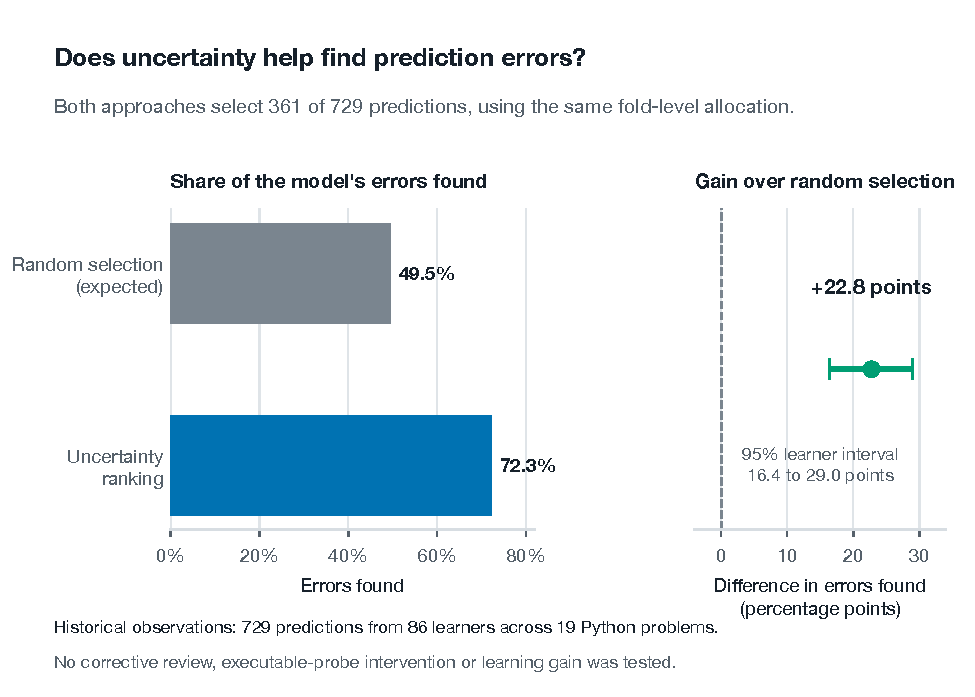
\includegraphics[width=\textwidth]{assets/figures/ch06-evaluation/uncertainty_error_review.pdf}
  \caption{Offline error prioritisation on 729 historical predictions from 86 learners across 19 Python problems. Selecting the
  most uncertain half within each fold, rounded down, captured 141/195 errors across 361 selected predictions. Random selection
  at the same fold allocations would capture 49.5\% in expectation. The gain was 22.8 percentage points (95\% learner bootstrap
  interval: 16.4 to 29.0). Larger values indicate more errors found. The interval conditions on fitted predictions and fixed
  selections. No review intervention, executable probe or learning effect was tested.}
  \label{fig:csedm-result}
\end{figure}

\FloatBarrier
\section{Local Computation and Its Measurement Limits}

The runtime records establish that the simulator work was practical on the development machine. They do not measure a
deployed tutor's response time. The tracker profile used CPython 3.12.13 on macOS with an ARM processor. The acquisition
profile additionally recorded ten logical CPUs and 16 GiB of physical memory. These are development measurements, separate
from the canonical scientific comparisons.

In the tracker timing study, each tracker processed 13,224 recorded updates with available evidence per repetition. An untimed validation pass established a reference checksum, followed by three warm-up repetitions and
twenty timed repetitions. Workload preparation was outside the timed region, and garbage collection was disabled during
measurement. Median time per update ranged from 1.55 microseconds for last-observation tracking to 2.94 microseconds for
bounded channel-aware updating. Ordinary channel-aware updating took 2.73 microseconds. The timed loop included update
invocation and checksum accumulation. These figures describe a prepared workload, not a full tutoring turn or an end-to-end
simulation. No statistical runtime superiority claim follows from them.

The probe selection study's compact development stream was measured in three fresh processes. Each processed 350 episodes across seven settings
and seven policies, producing 98,000 case predictions. Median elapsed time was 4.73 seconds. The largest observed process
peak resident memory was about 78.0 MiB. Timing began after plan loading and included stream generation, serialisation,
hashing and writing to a temporary file, including its final flush to storage. It excluded interpreter startup and downstream
analysis or figure generation. The recorded memory peak includes the process baseline, rather than measuring the policy alone.

Scaling that development time by forty produced a 189-second planning estimate for the canonical workload, or 379 seconds
with the declared factor-of-two allowance. Neither figure is a measured canonical duration. The canonical stream report
records 14,000 episodes, 3,920,000 case predictions across seven policies and 1,960,000 selected simulated probes, with zero
external-model or sandbox calls. These policy-level counts reuse the same episodes. They are not millions of independent
observations. Canonical runtime and peak memory are not recorded in that report and remain unavailable here.

% Sources: tracker development runtime fa5faaff4c604d185cb95486260f1afbceeadc96bd4b291d0dde4c840ce68540;
% acquisition compact runtime 47d0441452375510610b4b2a7e8c1b162e30a5d65896f7177cc9f3e425ec87b5;
% canonical stream cb13c0313c91c11a9cf39c79028180367534357fd6eac4394659e3a819851b60.

\section{What the Uncertainty Intervals Cover}
\suppressfloats[t]

Each interval describes variation under a particular analysis. Table~\ref{tab:interval-scope} states what was resampled
and what remained fixed. Pairing keeps the compared methods on the same cases or episodes. It does not remove limitations
in the data or the generating model.

\begin{table}[htbp]
  \centering
  \caption{Scope of the reported bootstrap intervals. Resampling changes the contribution of observed cases, episodes or
  learners to the estimate. It does not collect new model responses, create new failure settings or retrain the predictors.}
  \label{tab:interval-scope}
  \medskip
  \begin{tabularx}{\textwidth}{@{}>{\raggedright\arraybackslash}p{0.15\textwidth}>{\raggedright\arraybackslash}X>{\raggedright\arraybackslash}X@{}}
    \toprule
    Study & Resampled unit & Fixed inputs and excluded variation \\
    \midrule
    External model & Paired differences for the 23 eligible authored cases. & Recorded model responses, tracker and corrected checks. Case resampling does not account for shared concept families or variability from a new model run. \\
    \addlinespace
    Bounded updates & Paired effects for each episode. Turns are summarised within episodes. & Authored simulator rules and tracker settings. The interval does not describe new failure mechanisms or real learners. \\
    \addlinespace
    Probe selection & Paired episodes within each evaluation environment. Environment means receive equal weight. & Fitted calibration model, policies and six stress settings. Neither calibration refitting nor uncertainty about deployment frequencies is included. \\
    \addlinespace
    Learner records & Learners, keeping each learner's prediction records together. & Fitted predictions from the evaluation folds and selected review cases. Models are not retrained and cases are not ranked again. Dependence from overlapping training folds is not fully represented. \\
    \bottomrule
  \end{tabularx}
\end{table}

Adjusting the three primary probe-selection intervals for multiple comparisons leaves their scope conditional on the fitted
calibration and chosen environments. Development checks of calibration remain diagnostic. The CSEDM intervals likewise
exclude variability from retraining.

More simulated episodes can narrow an interval under the authored rules. They cannot establish that those rules describe
classroom behaviour. The external benchmark, simulations and historical learner analysis therefore retain separate conclusions.

\section{Answers to the Research Questions}

\begin{description}
  \item[RQ1: Extra coding evidence.] The corrected benchmark does not establish whether giving every case an extra coding
  check provides a useful prediction benefit. Accuracy changed from 18 to 19 correct predictions among 23 eligible authored
  cases. The paired interval, 0 to 13.04 percentage points, is too wide to rule in or rule out the declared ten-point useful
  improvement.

  \item[RQ2: Limiting a bad check.] The bounded update passed its prespecified simulator rule. Across the adverse settings,
  its mean Brier error was 0.0094 lower than ordinary channel-aware Bayes, while its clean-setting penalty was 0.0033. Missing
  and contradictory evidence still produced worse individual results, so bounding did not improve every condition.

  \item[RQ3: Choosing checks.] The proposed selector did not choose better cases than all three prespecified comparators at
  the fixed half-budget allocation. It beat random selection by 1.19 percentage points, but its error exceeded
  uncertainty-only selection by 0.86 points and the plug-in clipped-belief rule by 0.54 points. Because its score need not
  equal expected classification-error reduction, this result does not answer whether ordinary value-of-information selection
  would perform better.

  \item[RQ4: Finding likely errors.] In the exploratory CSEDM analysis, uncertainty found more existing prediction errors
  than random selection at the same allocation. It selected 141 of 195 errors, or 72.3\%, compared with 49.5\% expected under
  random selection. No corrective review was performed, so the result does not show that selecting these predictions would
  improve later performance.
\end{description}

% Working draft of discussion
\chapter{Discussion}
\label{ch:discussion}

The studies do not establish that more executable evidence generally improves prediction of programming performance. The external-model benchmark correction
showed that a measurement fault could create an apparently large benefit. The bounded-update study then showed that limiting one observation's influence
could help in a controlled tracker stress test. The probe-selection study showed the remaining difficulty: a cautious reliability model still selected
probes less effectively on the held-out average than uncertainty-only selection and the plug-in clipped-belief comparator.

The proposed selector's poorer performance supports keeping uncertainty-only selection as a baseline when testing more
complex rules. The result also shows why each rule needs a comparison under the conditions where it will be used.
Better reliability information and a different decision rule require further evaluation.

\section{What the Mathematical Review Changes}

Review after the experiment identified a gap between the acquisition score and the claimed expected classification benefit. Clipped
beliefs were substituted into a Bayes-risk expression even though they need not be the posterior of the generating model.
The counterexample in Chapter~\ref{ch:method} shows that the score can be positive when neither possible probe outcome changes
the predicted class. Ranking also evaluates hypothetical reliability-specific updates, while execution uses calibration means.

The experiment therefore evaluates the implemented ranking heuristic, not an exact value-of-information method. This narrows
the interpretation of its failure. It cannot establish that accounting for reliability uncertainty is generally ineffective,
or that a correctly specified expected-loss selector would also lose. Conversely, identifying the score limitation does not
establish that repairing it would improve the result. No such repair was evaluated in the frozen study.

The reference with access to true channel rates is similarly limited by its update and scoring rule. Its performance cannot
be used as a bound on the best achievable accuracy. The measured classification errors remain observations of the frozen
implementations. The report's corrected method descriptions preserve those observations.

\section{Alternative Explanations for the Negative Result}

The score mismatch is one possible contributor to the proposed selector's losses, but the experiment does not identify a single cause.
Uncertainty-only selection has an important advantage in this design: the supplied starting probabilities are calibrated,
so closeness to one half directly identifies cases with high initial classification risk. This gives the simple baseline
a useful signal before any reliability estimate is considered. It does not explain every ranking difference or establish
that the same advantage would persist with poorly calibrated starting probabilities.

The lower-quantile score may also down-rank useful checks when their reliability estimates are uncertain. That is the
intended caution mechanism, but caution is not automatically helpful at an exact allocation. The policy must still select
twenty cases. Rejecting one candidate moves the check to another. The study therefore cannot
separate a potentially useful refusal to probe from an unhelpful redistribution of a compulsory budget.

Clipping introduces another trade-off. It limits movement from a bad observation, but can prevent a useful observation from
changing a prediction. The development ablation varied clipping in both hypothetical scoring and executed updating, so it
does not isolate those two effects. Its small descriptive interaction offers no clear evidence that lower-quantile scoring
and clipping reinforce each other. A causal explanation of their respective contributions would require a separately
specified component study. The existing diagnostics are insufficient.

These alternatives change the interpretation of failure. The result rejects the proposed advantage for this combination
of data-generating rules, calibration fit, score and allocation. It does not isolate reliability uncertainty as the cause,
establish that a different quantile would succeed, or justify selecting a better-looking configuration after the fact.

\section{Contribution in Relation to Existing Methods}

Executable evidence and educational prediction were already connected in TIKTOC, while TRAVER examined verification in
coding-tutor dialogues \parencite{duan2025tiktoc,wang2025traver}. ECED supplies a theoretical treatment of sequential noisy-test
selection under explicit assumptions \parencite{chen2017noisy}. The dissertation neither replaces those methods nor provides
a common-benchmark comparison against them. Its combination of familiar components is not sufficient evidence of novelty.

The contribution is a documented analysis of failures in assessment and evidence selection. Predictions were retained before outcome reveal. Replay
exposed how a scoring fault changed the apparent effect. Controlled comparisons tested a proposed response to unreliable
evidence, and a mathematical check exposed a mismatch between the selector's score and its executed decision. Each step can
be examined separately. The value is the documented mechanism and the limits of the resulting claim, rather than a claim
that the pipeline or every safeguard is unprecedented.

This matters for future tutoring systems because choosing to collect more evidence adds another measurement process whose
quality must be checked. The present work gives concrete examples of that problem. It does not establish its prevalence,
show that these faults dominate deployed systems, or demonstrate that the proposed policy solves it.

\section{Selection, Updating and the Application Context}

At the full probe allocation, ordinary selectors request every case and apply the same bounded update. The harm at this
endpoint concerns the use of misleading evidence, independently of how cases are ranked. At smaller allocations, ranking
changes which cases receive that update. These are distinct questions, and a budget curve alone does not isolate every cause
of error.

The starting probabilities in the probe-selection study are calibrated by construction. Its primary result concerns evidence-channel failures,
not erroneous initial learner estimates. Selection is also performed once for a complete batch, with exactly 20 checks assigned
to each episode. The study does not demonstrate a tutor choosing its next question after each student answer, deciding to stop,
or adapting its teaching strategy over time.
Those capabilities remain application motivations rather than measured contributions.

The log-odds bound limits each observation's contribution. It does not prevent repeated misleading observations from accumulating
harm. The bounded-update study improved the adverse-condition average but worsened missing and contradictory conditions. Both results argue for
reporting condition-level failures alongside an aggregate, rather than interpreting a bounded update as a safety guarantee.

\section{What the Historical Data Add}

The exploratory CSEDM analysis asks whether the simplest selection signal remains useful beyond an authored simulator.
Here, the probabilities come from a logistic model fitted to historical learner activity. The analysis covers 729 predictions
from 86 learners across 19 Python problems.

Within the fixed fold-level allocations, selecting the 361 most uncertain predictions captured 141 of 195 model errors
(72.3\%). Random selection at the same allocation would capture 49.5\% in expectation. This provides evidence that
uncertainty can help locate prediction errors in these records, even though it does not explain how to correct them.

This is the connection to the earlier studies. The external-model benchmark tests the value of additional evidence, while
the simulations examine how evidence is interpreted and selected. The historical records test whether uncertainty identifies
where closer attention might be useful. They contain no matching optional-probe outcomes, so the result cannot validate the
probe-selection rule or establish that the simulator's failure settings reflect classrooms.

No reviewer intervened on the selected predictions. Error capture measures where errors were concentrated, rather than how many
could be corrected. Learner-separated folds assess predictions on the existing problem set. They do not test transfer to unseen
problems or courses. The small descriptive accuracy difference between the logistic model and problem-frequency baseline also
does not establish a meaningful predictive advantage by itself.

\section{Implications for Tutor Design}

An executable result needs an inspectable assessment record. The prompt, submitted code, tests, test output and task requirements
should remain linked so that a teacher or learner can see what was checked. The harness correction shows that repeatable execution
can still produce a misleading outcome when comparison logic or test coverage is wrong. A tutor should distinguish code that
failed to run, code that ran and failed a test, and code that passed incomplete tests. It should also provide a route for disputing
the interpretation.

The prediction update should expose its basis. A reviewer should be able to see the previous estimate, the evidence category,
the assumed reliability and the resulting decision. Bounding one update can limit the effect of a bad observation, but the
simulation shows that it can also discard useful information and that repeated errors can accumulate. Simple comparators such as
uncertainty-only selection should remain part of evaluation whenever a more elaborate policy is introduced.

Programming evidence can contain personal work, identifiers or sensitive context. Sending it to an external model and executing
it in a remote sandbox create separate data and security risks. A deployed system would need clear data destinations, limited
retention, deletion arrangements and isolated execution. The recorded fallback keeps the demonstration available during service
failure. Accepting untrusted public submissions would require a separate security design. These concerns sit alongside the transparency, privacy and
beneficence issues identified in reviews of educational LLM systems \parencite{yan2024practical}.

Repeated checks also use learner time. Their burden may fall unevenly if prediction errors differ across prior experience,
language background, disability or access conditions. Before classroom use, the system would need accessible alternatives,
subgroup error analysis and teacher oversight of disputed or high-consequence decisions. The scores studied here provide no
basis for grading a learner, withholding teaching or deciding that a concept has been mastered.

\section{Changes from the Proposal}

The original proposal joined a Socratic multi-agent tutor, a cognitively constrained student simulator, hidden-state tracking and
reinforcement-learning policy evaluation. That design required credible measurements of learning and cognitive load before
its policy results could be interpreted. The first implementation decision was therefore to establish a working tutoring path
and test whether its evidence could support a reliable prediction. The later tracker, acquisition and historical-data studies

% Address reviewer concern: why did Huber bounds help while greedy selection failed?

\chapter{Conclusion}
\label{ch:conclusion}

% Final summary and future work.


\printbibliography[heading=bibintoc,title={References}]

\appendix

\end{document}
